\documentclass[9pt]{sigplanconf}
\usepackage{etex}
\usepackage{float}
\usepackage{mathrsfs}
\usepackage{booktabs}
\usepackage{boxedminipage}
\usepackage[T1]{fontenc}
%\usepackage[pdf]{pstricks}
\usepackage{epsfig}
\usepackage{multirow}
\usepackage{url}
\usepackage[normalem]{ulem}
\usepackage{schemepgm}
\usepackage{graphicx}
\usepackage{graphpap}
\usepackage{tabularx}
\usepackage [plain,noend,noline,boxed]{algorithm2e}
\usepackage{amssymb}
\usepackage{amsmath}
\usepackage{pstricks}
\usepackage{pst-text}
\usepackage{pst-node}
\usepackage{pst-tree}
\usepackage{pst-rel-points}
\usepackage{bcprules}
%\usepackage{program}
\usepackage{algorithmic}


%%%%%%%%%% IMPERATIVE %%%%%%%%%%%%

%%%%%%%%%%%%%%%%%%%%%%%%%%%%%%%%%%%%%%%%%%%%%%%%%%%%%%%%%%%%%%%%%%
%%% Comment out a part of latex document
\newcommand{\cmt}[1]{}
\newcommand{\akadd}[1]{\protect{\red  #1}}
\newcommand{\akdel}[1]{\protect{\blue #1}}
\newcommand{\del}[1]{\protect{\magenta #1}}

\newcommand{\mybox}{\hfill\ensuremath{\Diamond}}
\newcommand{\NDIn}[1]{\mbox{\sf In$_#1$}}
\newcommand{\NDOut}[1]{\mbox{\sf Out$_#1$}}
%\newcommand{\x}{\cx}
%\newcommand{\y}{\cy}
%%%%%%%%%%%%%%%%%%%%%%%%%%%%%%%%%%%%%%%%%%%%%%%%%%%%%%%%%%%%%%%%%%

%%%%%%%%%%%%%%%%%%%%%%%%%%%%%%%%%%%%%%%%%%%%%%%%%%%%%%%%%%%%%%%%%%
%%%% Programs in latex 
\protect{\newlength{\FTABL}}
\protect{\newlength{\TABL}}
\protect{\newlength{\BRACE}}
\settowidth{\BRACE}{\{}

%%%%%%%%%%%%%%%%%%%%%%%%%%%%%%%%%%%%%%%%%%%%%%%%%%%%%%%%%%%%%%%%%%

 \newcommand{\ntbar}{\ensuremath{\overline\nt}}
%% %%%%%%%%%%%%%%%%%%%%%%%%%%%%%%%%%%%%%%%%%%%%%%%%%%%%%%%%%%%%%%%%%%
%%% Special pictures
\newcommand{\myarrow}{\mbox{%
 \psset{unit=1cm}%
 \begin{pspicture}(0,0)(.27,.2)%
  \psline[linewidth=.15mm]%
  (0,.1)(.125,.1)(.125,.035)(.25,.1)(.125,.165)(.125,.1)%
  \end{pspicture}}%
} 



%%
%% paths and derefs
\newcommand{\epath}{\mathsf{ep}}
\newcommand{\paths}{{\sf paths}}
\newcommand{\dpaths}{{\sf dpaths}}
\newcommand{\Pf}[2]{\ensuremath{\Pfonly_{\!\!#1}^{\,#2}}}
\newcommand{\Pfonly}{\ensuremath{\mathsf{PF}}}
\newcommand{\Pp}[2]{\ensuremath{\Pponly_{\!\!#1}^{\,#2}}}
\newcommand{\Pponly}{\ensuremath{\mathsf{PP}}}
\newcommand{\Pe}[3]{\ensuremath{\Peonly(#1, #2, #3)}}
\newcommand{\Peonly}{\ensuremath{\mathsf{PE}}}
\newcommand{\Peb}[3]{\ensuremath{\Pebonly(#1, #2, #3)}}
\newcommand{\Pebonly}{\ensuremath{\Peonly!}}
\newcommand{\Pv}{\ensuremath{\mathsf{P}}}
\newcommand{\Pvphi}{\ensuremath{\Pv^\emptyset}}
\newcommand{\Ddf}[2]{\ensuremath{\Ddfonly_{\!\!#1}^{\,#2}}}
\newcommand{\Ddfonly}{\ensuremath{\mathsf{DF}}}
\newcommand{\Dp}[2]{\ensuremath{\Dponly_{\!\!#1}^{\,#2}}}
\newcommand{\Dponly}{\ensuremath{\mathsf{DP}}}
\newcommand{\De}[3]{\ensuremath{\Deonly(#1, #2, #3)}}
\newcommand{\Deonly}{\ensuremath{\mathsf{DE}}}
%%\newcommand{\Deb}[3]{\ensuremath{\Debonly(#1, #2, #3)}}
%%\newcommand{\Debonly}{\ensuremath{\Deonly!}}
\newcommand{\Dv}{\ensuremath{\mathsf{D}}}
\newcommand{\Dvphi}{\ensuremath{\Dv^\emptyset}}
\newcommand{\derefs}{{\sf derefs}}

\newcommand{\bw}[1]{\ensuremath{\overline{#1}}} % backward
\newcommand{\cat}[2]{\ensuremath{#1#2}} % concat
\newcommand{\expshare}{\ensuremath{\mathsf{ExpS}}} % generic path

%% heap location and heap cell
\newcommand{\loc}[1]{\ensuremath{\mbox{\sf Loc}[{#1}]}}
\newcommand{\cell}[1]{\ensuremath{\mbox{\sf Cell}[{#1}]}}

%% type of labels
\newcommand{\acar}{\ensuremath{\mathbf{0}}}
\newcommand{\acdr}{\ensuremath{\mathbf{1}}}
\newcommand{\bcar}{\ensuremath{\bar\acar}}
\newcommand{\bcdr}{\ensuremath{\bar\acdr}}
\newcommand{\clazy}{\ensuremath{{\mathbf{2}}}}
\newcommand{\bX}  {\ensuremath{\bar{X}}}
\newcommand{\acarset}{\ensuremath{\lbrace\acar\rbrace}}
\newcommand{\acdrset}{\ensuremath{\lbrace\acdr\rbrace}}
\newcommand{\bcarset}{\ensuremath{\lbrace\bcar\rbrace}}
\newcommand{\bcdrset}{\ensuremath{\lbrace\bcdr\rbrace}}
\newcommand{\epsilonset}{\ensuremath{\lbrace\epsilon\rbrace}}

%%  transfer eqns - alias
\newcommand{\Af}[2]{\ensuremath{\Afonly_{#1}^{\,#2}}}
\newcommand{\Afonly}{\ensuremath{\mathsf{SF}}}
\newcommand{\Ap}[2]{\ensuremath{\Aponly_{#1}^{\,#2}}}
\newcommand{\Aponly}{\ensuremath{\mathsf{SP}}}
\newcommand{\Ae}[3]{\ensuremath{\Aeonly(#1, #2, #3)}}
\newcommand{\Aeonly}{\ensuremath{\mathsf{SE}}}
\newcommand{\Aa}[2]{\ensuremath{\Aaonly(#1, #2)}}
\newcommand{\Aaonly}{\ensuremath{\mathsf{SS}}}
\newcommand{\Av}{\ensuremath{\mathsf{S}}}
\newcommand{\Aphi}{\ensuremath{\Av^\emptyset}}
\newcommand{\Dfonly}{\ensuremath{\mathsf{D}}}
\newcommand{\Ufonly}{\ensuremath{\mathsf{I}}}
%\newcommand{\calls}[2]{\ensuremath{{\mathit{\!c}_{{\mathit #1}_#2}}}}
\newcommand{\calls}[2]{\ensuremath{{\mathit{\!c}_{{\mathit #1}}^#2}}}
%%\newcommand{\calls}[2]{\ensuremath{{\overline{\mathit #1}_{#2}}}}
%%  transfer eqns - liveness
\newcommand{\Uf}[2]{\ensuremath{\mathsf{I}_{\mathit #1}^{#2}}}
\newcommand{\Lfun}[3]{\ensuremath{\mathcal{L}(#1,#2,#3)}}
\newcommand{\Lfunonly}{\ensuremath{\mathcal{L}}}

\newcommand{\Df}[2]{\ensuremath{\mathsf{D}_{\mathit #1}^{#2}}}


\newcommand{\Lf}[3]{\ensuremath{\Lfonly_{\mathit #1}^{#2}( {\mathit #3})}}
\newcommand{\Lfonly}{\ensuremath{\mathsf{LF}}}
\newcommand{\Lfone}[1]{\ensuremath{\Lfonly_{\mathit #1}}}
\newcommand{\Le}[1]{\ensuremath{\Leonly({\mathit #1})}}
\newcommand{\Leonly}{\ensuremath{\mathsf{LE}}}
\newcommand{\Lp}[2]{\ensuremath{\Lponly_{#1}^{\,#2}}}
\newcommand{\Lponly}{\ensuremath{\mathsf{LP}}}
\newcommand{\Ld}[3]{\ensuremath{\Ldonly_{\mathit #1}^{#2}( {\mathit #3})}}
\newcommand{\Ldonly}{\ensuremath{\mathsf{LD}}}
\newcommand{\Lvc}[2]{\ensuremath{\Lv_{\mathit #1}^{\mathit #2}}}

\newcommand{\Lv}{\ensuremath{\mathsf{L}}}
\newcommand{\Lvphi}{\ensuremath{\Lv^\emptyset}}
\newcommand{\Leb}[3]{\ensuremath{\Lebonly(#1, #2, #3)}}
\newcommand{\Lebonly}{\ensuremath{\Leonly!}}
\newcommand{\NFA}{\mbox{\sf nfa}}
\newcommand{\lang}[1]{\ensuremath{\mathscr{L}({#1})}}
\newcommand{\Lan}[1]{\ensuremath{\Lv_{{#1}}}}
\newcommand{\Lanv}[2]{\ensuremath{\Lv_{{#1}}^{#2}}}
\newcommand{\dfa}[2]{\ensuremath{\mathsf{dfa}_{{#1}}^{#2}}}
%%  transfer eqns - availability
\newcommand{\AVf}[2]{\ensuremath{\AVfonly_{#1}^{\,#2}}}
\newcommand{\AVfonly}{\ensuremath{\mathsf{AvF}\,}}
\newcommand{\AVp}[2]{\ensuremath{\AVponly_{#1}^{\,#2}}}
\newcommand{\AVponly}{\ensuremath{\mathsf{AvP}\,}}
\newcommand{\AVgp}[2]{\ensuremath{\AVgponly_{#1}^{\,#2}}}
\newcommand{\AVgponly}{\ensuremath{{\mathsf{AvBP}}}}
\newcommand{\AVgf}[2]{\ensuremath{\AVgfonly_{#1}^{\,#2}}}
\newcommand{\AVgfonly}{\ensuremath{{\mathsf{AvBF}\,}}}
\newcommand{\AVe}[3]{\ensuremath{\AVeonly(#1, #2, #3)}}
\newcommand{\AVeonly}{\ensuremath{\mathsf{AvE}\,}}
\newcommand{\AVv}{\ensuremath{\mathsf{AV}}}
%\newtheorem{observation}[theorem]{Observation}

%%  transfer eqns - anticipability
\newcommand{\ANf}[2]{\ensuremath{\ANfonly_{#1}^{\,#2}}}
\newcommand{\ANfonly}{\ensuremath{\mathsf{AnF}}}
\newcommand{\ANp}[2]{\ensuremath{\ANponly_{#1}^{\,#2}}}
\newcommand{\ANponly}{\ensuremath{\mathsf{AnP}}}
\newcommand{\ANgp}[2]{\ensuremath{\ANgponly_{#1}^{\,#2}}}
\newcommand{\ANgponly}{\ensuremath{{\mathsf{AnBP}}}}
\newcommand{\ANgf}[2]{\ensuremath{\ANgfonly_{#1}^{\,#2}}}
\newcommand{\ANgfonly}{\ensuremath{{\mathsf{AnBF}}}}
\newcommand{\ANe}[3]{\ensuremath{\ANeonly(#1, #2, #3)}}
\newcommand{\ANeonly}{\ensuremath{\mathsf{AnE}}}
\newcommand{\ANv}{\ensuremath{\mathsf{AN}}}
\newcommand{\ANvphi}{\ensuremath{\ANv^\emptyset}}
\newcommand{\mmap}[3]{\ensuremath{\mathcal{M}_{\mathit{#1}}(\mathit{#2})(\mathit{#3})}}
\newcommand{\pmap}[1]{\ensuremath{\mathcal{P}_{\mathit{#1}}}}
\newcommand{\deltacall}[3]{\delta_{#1}({#2},{#3})}
%% union?
\newcommand{\plus}{$\cup$}

%% -> arrows, =def
\newcommand{\rightk}[1]{\ensuremath{\stackrel{\scriptstyle #1}{\rightarrow}}}
\newcommand{\rightstar}{\rightk{\star}}
%\newcommand{\eqdef}{\ensuremath{\stackrel{\scriptstyle def}{=}}}
\newcommand{\eqdef}{\ensuremath{=}}

%% functions

\newcommand{\listc}{\mbox{\tt l}}
\newcommand{\lista}{\mbox{\tt l1}}
\newcommand{\listb}{\mbox{\tt l2}}

%% nfa and cfg
\newcommand{\nfa}{\ensuremath{\mathbf{N}}}
\newcommand{\nfabar}{\ensuremath{\overline\nfa}}

\newcommand{\start}{{\sf init}}
\newcommand{\prim}{\ensuremath{P}}
\newcommand{\exit}{{\sf pgm}}
\newcommand{\gram}{\ensuremath{G}}
\newcommand{\nt}{\ensuremath{N}}
\newcommand{\var}[1]{\ensuremath{\langle #1\rangle}}

\newcommand{\TwoCells}[2]{%
\psset{unit=.25mm}
\begin{pspicture}(0,-2)(36,18)
\psframe(0,-5)(36,15)
\psline(18,-4)(18,15)
\putnode{zarb1342}{origin}{9}{5}{\rnode{#1}{}}
\putnode{zarb0102}{origin}{27}{5}{\rnode{#2}{}}
\end{pspicture}%
}

\newcommand{\TwoCellNull}[2]{%
\psset{unit=.25mm}
\begin{pspicture}(0,-2)(36,18)
\psframe(0,-5)(36,15)
\psline(18,-4)(18,15)
\psline(18,-4)(36,15)
\putnode{z}{origin}{9}{5}{\rnode{#1}{}}
\putnode{z}{origin}{27}{5}{\rnode{#2}{}}
\end{pspicture}%
}

\newcommand{\TwoCellsD}[2]{%
\psset{unit=.25mm}
\begin{pspicture}(0,-2)(36,18)
\psframe(0,-5)(36,15)
\psline(18,-4)(18,15)
\putnode{z}{origin}{9}{5}{\rnode{#1}{}}
\putnode{z}{origin}{27}{5}{\rnode{#2}{}}
\putnode{z}{origin}{9}{5}{%
      \psframebox[linestyle=none,fillstyle=hlines,hatchsep=2,framesep=8,
      hatchcolor=blue]{}}
\end{pspicture}%
}
\newcommand{\TwoCellsA}[2]{%
\psset{unit=.25mm}
\begin{pspicture}(0,-2)(36,18)
\psframe(0,-5)(36,15)
\psline(18,-4)(18,15)
\putnode{z}{origin}{9}{5}{\rnode{#1}{}}
\putnode{z}{origin}{9}{5}{%
   \psframebox[linestyle=none,fillstyle=hlines,hatchsep=2,framesep=8,
   hatchcolor=blue]{}}
\putnode{z}{origin}{27}{5}{\rnode{#2}{}}
\end{pspicture}%
}
\newcommand{\TwoCellsAD}[2]{%
\psset{unit=.25mm}
\begin{pspicture}(-6,-2)(42,18)
%\psframe(0,-5)(36,15)
%\psline(18,-4)(18,15)
\putnode{z}{origin}{9}{5}{\rnode{#1}{}}
\putnode{z}{origin}{9}{5}{%
   \psframebox[linestyle=none,fillstyle=solid,framesep=8,
   fillcolor=lightgray]{}}
\putnode{z}{origin}{27}{5}{%
      \psframebox[linestyle=none,fillstyle=solid,framesep=8,
   fillcolor=lightgray]{}}
\psccurve[fillstyle=solid,fillcolor=lightgray,linecolor=black]
(0,-5)(-6,5)(0,15)(12,20)(24, 15)(30,17)(36,15)(42,5)(36,-5)(24, -10)(12, -5)(6, -8)
\end{pspicture}%
}
% meta scheme command
\newcommand{\MIF}{\mbox{$\mathsf{if}$}}
\newcommand{\MEQ}{\mbox{$\mathsf{eq?}$}}
\newcommand{\MLET}{\mbox{$\mathsf{let}$}}
\newcommand{\MIN}{\mbox{$\mathsf{in}$}} 
%\newcommand{\IF}{\mbox{$\mathsf{if}$}}
%\newcommand{\SLET}{\mbox{$\mathsf{let}$}}
%\newcommand{\SIN}{\mbox{$\mathsf{in}$}} 

% others..
\newcommand{\candidates}[1]{\ensuremath{\mbox{\sf Candidates}(#1)}}
\newcommand{\scvars}[1]{\ensuremath{\mathsf{ScopeVars}(#1)}}
\newcommand{\expvars}[1]{\ensuremath{\mathsf{FV}(#1)}}
\newcommand{\mainpgm}{\ensuremath{\mathbf{main}}}
\newcommand{\main}{\ensuremath{\mathbf{main}}}
\newcommand{\updateenv}[3]{{\sf update(#1, #2, #3)}}
\newcommand{\pair}[2]{(#1, #2)}

\newcommand{\pia}{\ensuremath{\pi_{a}}}
\newcommand{\pib}{\ensuremath{\pi_{b}}}


\newenvironment{minieqnarray}
{\begin{minipage}{\textwidth}\begin{eqnarray}}
{\end{eqnarray}\end{minipage}}

%%% EFFECTIVENESS OF GC 
\newcommand{\deltarch}{\mbox{%
 \ensuremath{\delta_{\mbox{\footnotesize\sf rch}}}}}
\newcommand{\deltagc}{\mbox{%
 \ensuremath{\delta_{\mbox{\footnotesize\sf gc}}}}}
\newcommand{\GCstructure}{{\tt GC\_structure}}
\newcommand{\GCflag}{{\tt GC\_flag}}
\newcommand{\CreateTime}{{\tt Create\_time}}
\newcommand{\UseTime}{{\tt Use\_time}}
\newcommand{\CollTime}{{\tt Collection\_time}}
\newcommand{\exectime}{\mbox{\sf  T}}

\newcommand{\manual}[1]{{\protect#1}}

%% Benchmark names
\newcommand{\silex}{\mbox{\tt silex}}
\newcommand{\lalr}{\mbox{\tt lalr}}
\newcommand{\eopl}{\mbox{\tt eopl}}
\newcommand{\prolog}{\mbox{\tt prolog}}
\newcommand{\sudoku}{\mbox{\tt sudoku}}
\newcommand{\cipher}{\mbox{\tt cipher}}

%% helpful definitions
%%\renewcommand{\citeNP}{\cite}
\newcommand{\figtwo}{figure*}
\newcommand{\capsize}{}
\newcommand{\figrule}{}
\newcommand{\figtworule}{}

%% scheme program vars/constants
%% \renewcommand{\px}{\mbox{$\mathbf{x}$}}
%% \renewcommand{\py}{\mbox{$\mathbf{y}$}}
%% \renewcommand{\pz}{\mbox{$\mathbf{z}$}}
%% \renewcommand{\pw}{\mbox{$\mathbf{w}$}}
%% \newcommand{\pthree}{\mbox{$\mathbf{3}$}}
%% \newcommand{\pfour}{\mbox{$\mathbf{4}$}}
%% \newcommand{\pfive}{\mbox{$\mathbf{5}$}}
%% \newcommand{\psix}{\mbox{$\mathbf{6}$}}
%% \newcommand{\ptwo}{\mbox{$\mathbf{2}$}}
%% \newcommand{\append}{\mbox{$\mathbf{append}$}}
%% \newcommand{\set}{\mbox{$\mathbf{set{\mbox{\rm \bf !}}}$}}
%% \newcommand{\setcar}{\mbox{$\mathbf{set{\mbox{\rm \bf -}}car{\mbox{\rm \bf !}}}$}}
%% \newcommand{\setcdr}{\mbox{$\mathbf{set{\mbox{\rm \bf -}}cdr{\mbox{\rm \bf !}}}$}}

%% other defs
\newcommand{\nullifiable}{\mbox{\sf Nullifiable}}
\newcommand{\properprefix}{\mbox{\sf ProperPrefix}}
\newcommand{\prefix}{\mbox{\sf  Prefix}}
\newcommand{\linknull}{{\sf LinkNullify}}
\newcommand{\pathnullify}{{\sf PathNullify}}
\newcommand{\nullins}{{\sf GenNullCode}}
\newcommand{\nullstatements}{\mbox{\sf null-statements}}
\newcommand{\isnull}{\mbox{\sf isnull}}
\newcommand{\mymark}{\mbox{\sf Mark}}
\newcommand{\sbegin}{\mbox{\sf BEGIN}}
\newcommand{\map}{\mbox{\sf map}}
\newcommand{\nullset}{\ensuremath{\mathsf{N}}}
\newcommand{\insnull}[2]{\mbox{$\mathsf{InsertNull(#1,#2)}$}}  
\newcommand{\insnullfn}{\mbox{$\mathsf{InsertNull}$}}   

\newcommand{\compnullfn}{\mbox{$\mathsf{Nullify}$}} 
\newcommand{\compnull}[2]{\compnullfn(#1, #2)}
\newcommand{\compnullpgm}[1]{\mbox{$\mathsf{Nullifypgm(#1)}$}}
\newcommand{\compnulldef}[1]{\mbox{$\mathsf{Nullifydef(#1)}$}}

\newcommand{\zz}{{\sf z}}
\newcommand{\yy}{{\sf y}}
\newcommand{\xx}{{\sf x}}
\newcommand{\ww}{{\sf w}}
\newcommand{\uu}{{\sf u}}
\newcommand{\aap}{{\sf a}}
\newcommand{\result}{{\sf result}}

%% \newtheorem{lemma}{Lemma}[section]
%% \newtheorem{example}{Example}[section]
%% \newtheorem{theorem}{Theorem}[section]
%% \newtheorem{definition}{Definition}[section]
%% \newtheorem{corollary}{Corollary}[section]
%% \newtheorem{property}{Property}[section]
%% \newcommand{\qed}{\hfill\nobreak \ifvmode \relax \else
%%   \ifdim\lastskip<1.5em \hskip-\lastskip
%%   \hskip1.5em plus0em minus0.5em \fi \nobreak
%%   \vrule height0.75em width0.5em depth0.25em\  fi}
\newcommand{\qed}{\hfill\ensuremath{\square}}
 \newenvironment{proof}[1][Proof]{\begin{trivlist}
 \item[\hskip \labelsep {\bfseries #1}]}{\hfill\qed\end{trivlist}}

\newcommand{\expr}[1]{\ensuremath{#1}}
%\newcommand{\pv}[1] {\mbox{\tt #1}}
\newcommand{\db}[1]{{\bf [\![}#1{\bf ]\!]}}
\newcommand{\nat}{I\!\!N}
\newcommand{\lenprime}{\ \vdash^{l'}\ }
\newcommand{\len}{\ \vdash^l\ }
\newcommand{\sen}{\ \vdash^s\ }
\newcommand{\fen}{\ \vdash^f\ }
\newcommand{\den}{\ \vdash^f\ }
\newcommand{\argsen}{\ \vdash^{args}\ }
\newcommand{\pen}{\ \vdash^p\ }
\newcommand{\fsen}{\ \vdash^{fs}\ }
\newcommand{\psen}{\ \vdash^{ps}\ }

\newcommand{\last}{\mbox{last}}
\newcommand{\rightmost}{\mbox{rightmost}}
\newcommand{\before}{\mbox{before}}
\newcommand{\befen}{\ \vdash^{\sf before}}
\newcommand{\lasten}{\ \vdash^{\sf last}}
\newcommand{\rmen}{\ \vdash^{\sf rightmost}}
\newcommand{\rhos}{\ensuremath{\red \rho_s}}
\newcommand{\pgmpt}[1]{\ensuremath{\red \pi_{#1}}}
\newcommand{\multireduct}{\ensuremath{\stackrel{+}{\longrightarrow}}}
\newcommand{\avrightarrow}{\ensuremath{\longrightarrow}}
\newcommand{\multireductav}{\ensuremath{\stackrel{+}{\avrightarrow}}}
\newcommand{\heap}{\ensuremath{H}}       % heap
\newcommand{\ppn}[2]{\ensuremath{#2}} % prog point
\newcommand{\pp}[2]{\ensuremath{#2}} % prog point
\newcommand{\lvintp}{\ensuremath{\zeta}}
\newcommand{\avintp}{\lvintp}
\newcommand{\locs}{\mbox{\tt locs}} 
\newcommand{\llv}{\ensuremath{\mathcal{L}}}
\newcommand{\aav}{\ensuremath{\mathcal{A}}}
\newcommand{\aan}{\ensuremath{\mathcal{N}}}
\newcommand{\gl}{\mbox{\em G}}




\def\drawplusplus#1#2#3{\hbox to 0pt{\hbox to #1{\hfill\vrule height #3 depth
      0pt width #2\hfill\vrule height #3 depth 0pt width #2\hfill
      }}\vbox to #3{\vfill\hrule height #2 depth 0pt width
      #1 \vfill}}
      %Poor man's typography
\def\concat{\mathrel{\drawplusplus {12pt}{0.4pt}{5pt}}}
      %It would be better to specify these in font-relative measures, but it
      %probably doesn't scale anyway.
\newcommand{\mycomment}[1]{}
\definecolor{Myblue}{rgb}{.2,0,1}
\newcommand{\comment}[1]{{\color{Myblue}{(#1)}}}
\newcommand{\cred}[1]{{\color{red}{#1}}}
\newcommand{\alan}[1]{{\color{red}{\medskip \hrule\medskip
    #1 \medskip \hrule \medskip}}}
\newcommand{\blankout}[1]{}


%\newcommand{\deltacall}[3]{\delta_{#1}({#2},{#3})}
\newcommand{\scmin} {\mbox{\sf\em in}}
\newcommand{\scmnull}{\mbox{\sf\em null?}}
\newcommand{\scmpair}{\mbox{\sf\em pair?}}
\newcommand{\scmprim}{\ensuremath{\mathsf{+}}}
\newcommand{\sh}[1]{{\colorbox{gray!20}{\framebox{$#1$}}}}
\def\myvec{\mathaccent"017E } % wretched springer mode redefines \vec as bold!
\newcommand{\stk}{\mbox{S}}       % stack
\newcommand{\ID}{\mbox{$\mathbf{ id}$}} % identity function
\newcommand{\bang}{\mbox{\sc bang}}
\newtheorem{theorem}{Theorem}[section]
\newtheorem{proposition}[theorem]{Proposition}
\newtheorem{definition}[theorem]{Definition}
\newtheorem{lemma}[theorem]{Lemma}
\begin{document}
% --- Author Metadata here ---
\conferenceinfo{WOODSTOCK}{'97 El Paso, Texas USA}
%\CopyrightYear{2007} % Allows default copyright year (20XX) to be over-ridden - IF NEED BE.
%\crdata{0-12345-67-8/90/01}  % Allows default copyright data (0-89791-88-6/97/05) to be over-ridden - IF NEED BE.
% --- End of Author Metadata ---

\title{Liveness-Based Garbage Collection for Lazy Languages}

% You need the command \numberofauthors to handle the 'placement
% and alignment' of the authors beneath the title.
%
% For aesthetic reasons, we recommend 'three authors at a time'
% i.e. three 'name/affiliation blocks' be placed beneath the title.
%
% NOTE: You are NOT restricted in how many 'rows' of
% "name/affiliations" may appear. We just ask that you restrict
% the number of 'columns' to three.
%
% Because of the available 'opening page real-estate'
% we ask you to refrain from putting more than six authors
% (two rows with three columns) beneath the article title.
% More than six makes the first-page appear very cluttered indeed.
%
% Use the \alignauthor commands to handle the names
% and affiliations for an 'aesthetic maximum' of six authors.
% Add names, affiliations, addresses for
% the seventh etc. author(s) as the argument for the
% \additionalauthors command.
% These 'additional authors' will be output/set for you
% without further effort on your part as the last section in
% the body of your article BEFORE References or any Appendices.
\cmt{{
\numberofauthors{3} %  in this sample file, there are a *total*
% of EIGHT authors. SIX appear on the 'first-page' (for formatting
% reasons) and the remaining two appear in the \additionalauthors
section.
%
\author{
% 1st. author
\alignauthor K. Prasanna Kumar \\
       \affaddr{IIT Bombay,}\\
       \affaddr{Mumbai 400076, India}
       \email{prasanna@cse.iitb.ac.in}
% 2nd. author
\alignauthor Amey Karkare\\
       \affaddr{IIT Kanpur}\\
       \affaddr{Kanpur 208016, India}
       \email{karkare@cse.iitk.ac.in}
% 3rd. author
\alignauthor Amitabha Sanyal \\
       \affaddr{IIT Bombay}\\
       \affaddr{Mumbai 400076, India}\\
       \email{as@cse.iitb.ac.in}
}
}}
\authorinfo{Double Blind Review}{}{}
\maketitle



\begin{abstract}
We consider  the problem of reducing  the memory required  to run lazy
first-order functional programs.  To  do this, we analyze programs for
liveness of heap  allocated data, i.e. data that  can possibly be used
in the future.  The accompanying garbage collector is  modified to use
the result of the analysis to preserve only {\em live} data---a subset
of {\em reachable data}---during  garbage collection.  This results in
an  increase in  the garbage  reclaimed and  consequently  reduces the
memory footprints of programs.   While this technique has already been
shown to yield benefits  for eager first-order languages, the presence
of  closures   at  run-time  poses  additional   challenges  for  lazy
languages.   Closures require  changes  both in  the earlier  liveness
analysis for heap allocated memory  and also in the garbage collection
scheme required to reclaim memory that is not live.

We  formulate  a context-sensitive  liveness  analysis  and using  the
results annotate each potential allocation point in the program with a
set     of    deterministic    finite-state     automata(DFA).     The
garbage-collector  inspects  the DFA  to  curtail reachability  during
marking.  As a result, fewer  objects are marked (with a possibly more
expensive  marker)  and  preserved  by the  copy  phase.   Experiments
confirm  that  liveness-based  collection  results in  a  increase  in
garbage  reclaimed  and  a   consequent  decrease  in  the  number  of
collections. On  our benchmark programs, we obtain  a decrease between
x\% and y\% in the memory size required to run programs, when compared
to reachability-based garbage collection.
\end{abstract}

% A category with the (minimum) three required fields
\category{H.4}{Information Systems Applications}{Miscellaneous}
%A category including the fourth, optional field follows...
\category{D.2.8}{Software  Engineering}{Metrics}[complexity  measures,
  performance measures]

\terms{Theory}

\keywords{ACM proceedings, \LaTeX, text tagging}

By Friday, February 27 2015, 23:59 (UTC-11), submit a full paper of at
most  12 pages (6  pages for  an Experience  Report), in  standard ACM
conference format, including bibliography, figures, and appendices.

\section{Introduction}
\label{sec:intro}

Functional programs extensively use dynamically allocated memory.  The
allocation  is either  explicit (for  example, using  constructors) or
implicit  (during creation  of  closures).  Programs  written in  lazy
functional languages put additional  demands on memory as they require
closures to  be carried  from the  point of creation  to the  point of
evaluation.

While  the runtime  system  of most  functional  languages includes  a
garbage collector to efficiently  reclaim memory, empirical studies on
Scheme~\cite{karkare06effectiveness}   and,   more   importantly,   on
Haskell~\cite{rojemo96lag}
%and Java~\cite{shaham02estimating}
programs have shown that  garbage collectors leave uncollected a large
number of  memory objects that are  reachable but not  live (here {\em
  live} means the  object can potentially be used by  the program at a
later stage).  This results in unnecessary memory retention.

%%%%%%%%%%%%%%%%%%%%%%%%%%%%%%%%%%%%%%%%%%%%%%%%%%%%%%%%%%%%%%%%%%%%%%%
%%%%
%%% MOTIVATING EXAMPLE
\newcommand{\nilfigure}
{\scalebox{0.75}{
\psset{unit=1mm,nodesep=0mm,labelsep=0.5mm}
\begin{pspicture}(0,0)(1,1)
%\psgrid[xunit=1cm,yunit=1cm,gridwidth=.2pt,subgridwidth=.1pt,
subgriddiv=5,subgridcolor=gray,gridcolor=blue](0,0)(1,1)
\putnode{start}{origin}{0}{0}{}
\putnode{stop}{origin}{10}{10}{}
\ncline[offsetB=0,nodesepB=0,linewidth=.7]{-}{start}{stop} %here
\end{pspicture}
}}


\begin{figure*}[t!]
%%%%{\color{Myblue}
\begin{picture}(100,130)(0,-90)
%  \begin{center}
    \begin{tabular}{cc}
\begin{boxedminipage}{.42\textwidth}
      {\sf
	\renewcommand{\arraystretch}{1}{
	  \begin{uprogram}
          \UFL\
\UNL{0} (\DEFINE\ (\length\  \pl)
	  \UNL{1}  (\SIF~(\NULLQ \ \pl) $0$
          (\PRIM\ 1\ (\CAR\  \pl))))
           \UNL{0}
	   \UNL{0}  (\DEFINE\ (\append\  \lista\ \listb)
	  \UNL{1}  (\SIF~(\NULLQ \ \lista)
	       \listb
	  \UNL{2} \hspace*{-0.1cm}(\CONS\ (\CAR\  \lista) (\append\
(\CDR\  \lista)
          \listb))))
          \UNL{0}
          \UNL{0} (\LET\ \px\
          $\leftarrow$\ (\CONS\ $5$
%          \UNL{1}\hspace*{1.5cm}
          (\CONS\ (\CONS\ $6$ \NIL) \NIL) \IN
	  \UNL{1} (\LET\ \py\   $\leftarrow$\  (\CONS\ $3$ \NIL) \IN
	  \UNL{2}
          (\LET\ \pz\  $\leftarrow$\  (\append\ \px\  \py)\ \IN\
          \UNL{3} (\SIF~(\NULLQ~(\CAR~(\CDR~\pz)))~$0$~$\pi$:\
(\length\ \pz))))))
	\end{uprogram}
      }}
\end{boxedminipage}
&
\begin{minipage}{.45\textwidth}

\hspace*{1cm}{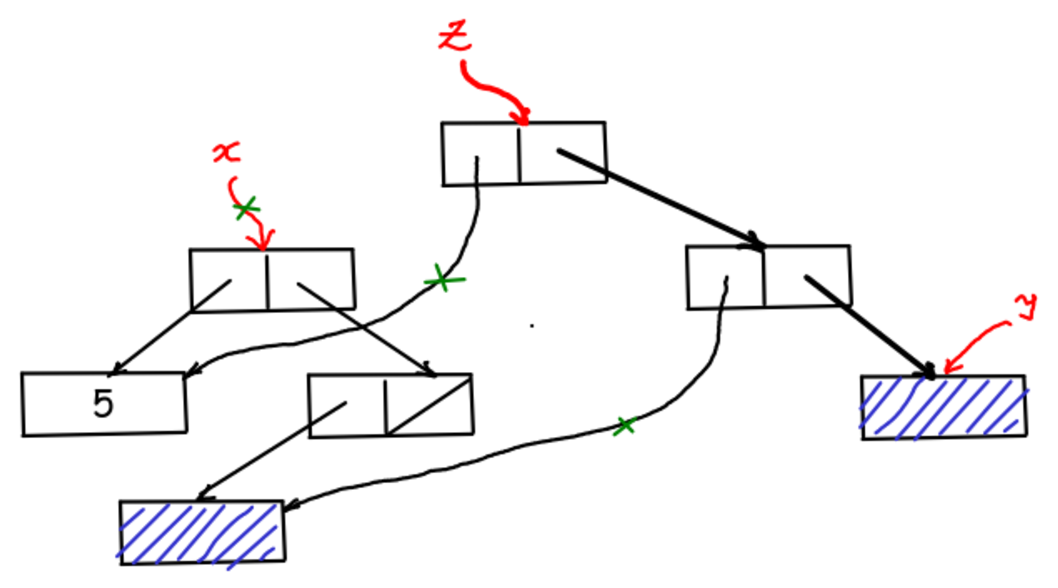
\epsfig{file=motiv-example.eps, height=4cm}}

\end{minipage}

\\

%%%%%%%%%%%%%%%%%%%%%%%%%%%%%%%%%%%%%%%%%%%%%%%%%%%%
%%       &
%%       \raisebox{-25mm}{\scalebox{.75}{
%% 	%%%%%%%%%%%%%%%%%%%%%Uday's stuff%%%%%%%%%%%%%%%%%%%%%%%%%
%%       \psset{unit=1mm}
%%       \psset{linewidth=.3mm}
%%       \begin{pspicture}(0,-5)(70,60)
%% 	%\psframe(0,0)(73,60)
%%
%%%%%%%%%%%%%%%%%%%%%%%%%%%%%%%%%%%%%%%%%%%%%%%%%%%%%%%%%%%%%%%%
%% 	\putnode{o}{origin}{13}{50}{\TwoCells{o1}{o2}}
%% 	\putnode{a}{o}{-10}{-15}{\psframebox{3}}
%% %
%%      \putnode{b}{o}{10}{-15}{\psframebox[linestyle=none,framesep=.5]{\NIL}}
%% 	\ncline[offsetB=-.5,nodesepB=.1]{*->}{o1}{a}
%%
%\aput[-3.5](.5){\scalebox{1.2}{\psframebox[framesep=.2,linestyle=none,
%%      fillstyle=solid,
%% 	%      fillcolor=white]{$\times$}}}
%%
%%  \putnode{b}{o}{0}{-3}{\psframebox[linestyle=none,framesep=.5]{\scalebox
%%{.63}{\nilfigure}}}
%% %	\ncline[offsetB=-.5,nodesepB=.1]{*->}{o2}{b}
%% 	%\ncline[offsetB=-.5,nodesepB=.1]{->}{o2}{b}
%%
%% \putnode{y}{o}{-14}{8}{\psframebox[linestyle=none,framesep=.5]{y}}
%% 	\nccurve[nodesepB=-.2,angleA=330,angleB=120]{->}{y}{o}
%%
%% \aput[-3.5](.5){\scalebox{1.2}{\psframebox[framesep=.2,linestyle=none,
%%fillstyle=solid,
%% 		  fillcolor=white]{$\times$}}}
%% 	%%%%%%%%%%%%%%%%%%%%%%%%%%%%%%%%%%%%%%%%%%%%%%%%%%%%%%
%% 	\putnode{c}{o}{25}{0}{\TwoCells{c1}{c2}}
%% 	\putnode{d}{c}{10}{-10}{\TwoCells{d1}{d2}}
%% 	\putnode{e}{d}{-13}{-12}{\TwoCells{e1}{e2}}
%% 	\putnode{f}{d}{13}{-12}{\TwoCells{f1}{f2}}
%% 	\ncline[nodesepB=-.5]{*->}{c2}{d}
%% 	\ncline[nodesepB=-.5,linewidth=.7]{->}{c2}{d}
%% 	\nccurve[ncurv=1,angleA=270,angleB=330]{*->}{c1}{a}
%%
%% \aput[-3.5](.2){\scalebox{1.2}{\psframebox[framesep=.2,linestyle=none,
%% fillstyle=solid,
%% 	      fillcolor=white]{$\times$}}}
%% 	\nccurve[nodesepB=-.5,angleA=240,angleB=70]{*->}{d1}{e}
%%
%% \nccurve[nodesepB=-.5,angleA=240,angleB=70,linewidth=.7]{->}{d1}{e}
%% 	\nccurve[nodesepB=-.5,angleA=300,angleB=110]{*->}{d2}{f}
%%
%% \aput[-3.5](.5){\scalebox{1.2}{\psframebox[framesep=.2,linestyle=none,
%% fillstyle=solid,
%% 	      fillcolor=white]{$\times$}}}
%%
%% \putnode{w}{c}{-8}{8}{\psframebox[linestyle=none,framesep=.2]{w}}
%%
%%\putnode{ww}{c}{15}{8}{\psframebox[linestyle=none,framesep=.2]{z}}
%%
%%\nccurve[nodesepB=-.2,angleA=330,angleB=120,linewidth=.7]{->}{w}{c}
%%
%%%%%%%%%%%%%%%%%%%%%%%%%%%%%%%%%%%%%%%%%%%%%%%%%%%%%%%%%%%%%%%%%%
%% 	\putnode{g}{e}{-8}{-12}{\psframebox{4}}
%% 	\putnode{h}{e}{8}{-14}{\TwoCells{h1}{h2}}
%% 	\putnode{i}{f}{-8}{-11}{\psframebox{6}}
%% %
%%\putnode{j}{f}{8}{-11}{\psframebox[linestyle=none,framesep=.5]{\NIL}}
%% 	\ncline[offsetB=-.5,nodesepB=.1]{*-}{e1}{e1}
%%
%%\ncline[linestyle=dashed,offsetB=-.5,nodesepB=.1,linewidth=.7]{->}{e1}{g}
%%         %here
%%
%%\putnode{j1}{f}{0}{-3}{\psframebox[linestyle=none,framesep=0]{\scalebox{.63}{\nilfigure}}}
%%
%%\putnode{j2}{h}{0}{-3}{\psframebox[linestyle=none,framesep=.5]{
%%\scalebox{.63}{\nilfigure}}}

%% %
%%\aput[-3.2](.6){\scalebox{1.2}{\psframebox[framesep=.1,linestyle=none,
%%fillstyle=solid,
%% %	      fillcolor=white]{$\times$}}} %and here
%% 	\ncline[offsetB=-.5,nodesepB=-.3]{*-}{e2}{e2}
%%
%%\ncline[linestyle=dashed,offsetB=-.5,nodesepB=.1,linewidth=.7]{->}{e2}{h}
%% %
%%\aput[-3.2](.5){\scalebox{1.2}{\psframebox[framesep=.1,linestyle=none,
%%fillstyle=solid,
%% %	      fillcolor=white]{$\times$}}} %and here

%% 	\ncline[offsetB=-.5,nodesepB=.1]{*->}{f1}{i}
%% 	\ncline[offsetB=-.5,nodesepB=.1]{*->}{f2}{j}
%% 	\nccurve[nodesepB=-.2,angleA=270,angleB=90]{->}{ww}{d}
%%
%%\aput[-3.2](.4){\scalebox{1.2}{\psframebox[framesep=.1,linestyle=none,fillstyle=solid,
%% 	      fillcolor=white]{$\times$}}}
%%
%%%%%%%%%%%%%%%%%%%%%%%%%%%%%%%%%%%%%%%%%%%%%%%%%%%%%%%%%%%%%%%%%%
%% 	\putnode{k}{h}{-8}{-11}{\psframebox{5}}
%% %
%%\putnode{l}{h}{8}{-11}{\psframebox[linestyle=none,framesep=.5]{\NIL}}
%% 	\ncline[offsetB=-.5,nodesepB=.1]{*-}{h1}{h1}
%%
%%\ncline[linestyle=dashed,offsetB=-.5,nodesepB=.1,linewidth=.7]{->}{h1}{k}
%% %	\ncline[offsetB=-.5,nodesepB=.1]{*->}{h2}{l}
%%
%%%%%%%%%%%%%%%%%%%%%%%%%%%%%%%%%%%%%%%%%%%%%%%%%%%%%%%%%%%%%%%%
        %%
%%       \end{pspicture}}} \\
%% %%%%%%%%%%%%%%%%%%%%%%%%%%%%%%


      (a) Example program.&\hspace*{2cm}
      \renewcommand{\arraystretch}{.9}{\begin{tabular}[t]{ll}
	(b) Memory graph at $\pi$. Thick edges denote  \\
        {\white (b) }live links. Traversal stops at edges marked\\
        {\white (b) }$\times$  during garbage collection.
      \end{tabular}}
    \end{tabular}
\end{picture}

\kern -3ex

\caption{Example Program and its Memory Graph.{\color{red}Amey will combine this with the figure for syntax}}\label{fig:mot-example}
\end{figure*}

In this paper,  we propose the use of liveness  analysis of heap cells
for garbage collection in a lazy first-order functional language.  The
central notion in our analysis  is a generalization of liveness called
{\em  demand}---the  pattern  of  future  uses  of  the  value  of  an
expression.   The analysis  has two  parts.  First,  each  function is
summarized in a context-sensitive manner as a {\em demand transformer}
that transforms a {\em symbolic} demand  on its body to demands on its
arguments.  This summary  is then used to step  through function calls
during analysis.   Second, the concrete  demand on a function  body is
obtained through a 0-CFA-like conservative approximation that combines
the  demands on  all the  calls to  the function.   The result  of the
analysis  is the annotation  of each  program point  with finite-state
automata capturing  the liveness of variables at  the point. Depending
on the program point where  garbage collection has been triggered, the
garbage-collector consults  a set of automata  to curtail reachability
during marking.  This results in  an increase in the garbage reclaimed
and consequently in fewer garbage collections.

While this idea has been shown to be effective~\cite{asati14lgc} for a
first-order {\em  eager} language, a straightforward  extension of the
earlier  technique  is  not  possible  for  lazy  languages,  where  a
heap-allocated  object may either  be an  unevaluated expression  or a
closure. Since  data is  made live by  evaluation of closures,  and in
lazy languages  the place in  the program where this  evaluation takes
place cannot  be statically determined,  laziness complicates liveness
analysis itself.  In  addition, apart from evaluated data,  we want to
extend  liveness-based collection also  to closures---closures with no
future use should also  be collected.  This involves tracking closures
to  their points of  creation at  runtime from  where we  obtain their
liveness.  This  requires significant  modification to the  earlier GC
scheme.

{\color  {Myblue}Rewrite after the experiments:  Experiments  with a
single
  generation  copying  collector   confirm  the  expected  performance
  benefits.   Liveness-based  collection  results  in an  increase  in
  garbage reclaimed.   As a  consequence, there is  a decrease  in the
  number of  collections and a  (some quantification) decrease  in the
  memory size required  to run programs. Besides there  is a reduction
  in the overall execution time for some programs.}


%------------------------------------------------------------%
\subsection{Motivating Example}
\label{sec:motiv}

Figure~\ref{fig:mot-example} shows an example program and the state of
the heap at the program point $\pi$, i.e. just before the  evaluation
of $(\length\ \pz)$.  The heap is represented by a graph in which
a node  either represents atomic values ($\NIL$,  integers etc.), or
a \CONS\  cell  containing $\CAR$  and  $\CDR$  fields, or a chunk of
memory representing an unevaluated
value  also called a  {\em closure}  (represented by  hatched boxes).
Edges in the graph are  {\em references} and emanate from variables or
fields.  The figure shows the lists \px\ and \pz\ partially evaluated.
The evaluation was triggered by the test (\NULLQ~(\CAR~(\CDR~\pz))) in
the \SIF\ expression.


The edges shown by thick arrows  are those which are live at $\pi$.  A
cell is marked and preserved  during garbage collection only if it is
reachable from the  root set through a path of  live edges.  All other
cells can be  reclaimed.  Thus if a garbage  collection takes place at
$\pi$ with the heap shown in Figure~\ref{fig:mot-example}(b), only the
cells referenced by $\pz$,  $(\CDR~ \pz)$ and (the cells constituting)
the closure  referenced by $(\CDR~(\CDR~\pz))$  need to be  marked and
preserved.  In  contrast, a  reachability-based  collector would  have
preserved all cells.

{\color {Myblue}Rewrite at the end: The  specific contributions of the
paper
  are: The formulation of a  liveness analysis for a lazy language and
  the proof of its correctness, the undecidability of the grammar that
  results from the analysis and  its approximation by DFAs, the design
  of a  garbage collector that can  use the DFAs to  retain live cells
  that  also include  closures, and  empirical results  that  show the
  effectiveness of liveness-based garbage collection.}

\subsection{Organization of the paper}

Section~\ref{sec:defs} introduces the syntax and semantics of the
language used to illustrate our
analysis.
% Section~\ref{sec:operational} describes the operational semantics of
% the language.
Liveness analysis for this language is  described in
Section~\ref{sec:liveness}. This section also has by  a  sketch  of  a
correctness proof  relative  to  a  non-standard
semantics.  Section~\ref{sec:computing}  shows how to  encode liveness
as   finite-state  automata.    Section~\ref{sec:experiments}  reports
experimental  results  and Section~\ref{sec:lgc-always-better}  proves
that a liveness based collector  can never do more garbage collections
than a reachability based collector.
% and Section~\ref{sec:conclusion} concludes the paper.

\section{The target language---syntax and semantics}
\label{sec:defs}
%%We let $x$, $y$, $z$ range over variables, $f$ over user-functions
and
%% $p$    over    primitive    functions   ($\CONS$,    $\PRIM$ etc.).
Figure~\ref{fig:lang-syntax} describes the  syntax of our language. It
is a first order language with lazy semantics. Programs are restricted
to        be        in        Administrative        Normal        Form
(ANF)~\cite{chakravarty03perspective}  where all actual  parameters to
functions  are  variables.  While  this  restriction  does not  affect
expressibility,  this form  has  the benefit  of  making explicit  the
creation  of closures through  the $\LET$  construct.  $\LET$s  in our
language  are lazy;  in the  expression $\LET\,\,  x  \leftarrow s\,\,
\IN\,\, e$, $x$ may occur  in $s$. This enables creation of graph-like
structures in  a pure language. The  restriction of \LET\  to a single
definition  is  for ease  of  exposition---generalization to  multiple
definitions  does  not add conceptual  difficulties.  We  further
restrict each variable  in a program to be distinct,  so that no scope
shadowing   occurs---this  simplifies   proofs   of  soundness.    The
$\SRETURN$ and \SIF\ expressions trigger evaluation of closures.

The body  of a function ${\mathit  f}$ is denoted  as $e_{\mathit f}$.
We   shall   extend   this   convention   to   the   main   expression
$e_\mainpgm$. We assume that each program has a distinguished function
\mainpgm\      with      the      definition     $(\DEFINE\      ({\tt
  \mainpgm})\  e_\mainpgm)$ and  the execution  of the  program starts
with the call to \mainpgm.  We write $\pi\!:\!e$ to associate the label
$\pi$ (not  part of the language  syntax) with the  program point just
before expression $e$.

% \paragraph{Inlining.}
{ \color {Myblue} Relook after proof: In spite of the  ANF restrictions
it
  is still possible  to inline non-recursive functions (a  fact we use
  to  prove the safety  of liveness  analysis).  A  user-function call
  $(\LET\,\, x \leftarrow (f\,y_1\,\ldots\,y_n)  \,\, \IN\,\, e)$ to a
  function  defined  (after renaming  its  formals  and  locals to  be
  disjoint         from         existing         variables)         by
  $(\DEFINE\ (f\ z_1\ \ldots\ z_n)\ e_f)$ is replaced by a sequence of
  $\LET$'s of  the form  $z_i\leftarrow (\ID\,\,y_i)$ followed  by the
  body $e_f$  but with  its $(\SRETURN\,\,w)$ expressions  replaced by
  $(\LET\,\, x \leftarrow (\ID\,\, w) \,\, \IN\,\, e)$.}

\begin{figure*}[]
\footnotesize
\begin{eqnarray*}
   p \in \mathit{Prog} & ::= & d_1 \ldots d_n \,\, e_\mainpgm
    \hspace{7em} \mbox{\em --- program}\\
    \mathit{df} \in Fdef & ::= & (\DEFINE\,\, (f\,\, x_1 \,\, \ldots \,\,x_n)\,\,
    e) 
    \hspace{2.2em} \ \ \ \ \mbox{\em --- function definition} \\
e \in \mathit{Expr} & ::= &
\left\{\begin{array}{ll@{\hspace{4em}}l}
       (\SIF\,\, x\,\, e_1\,\, e_2) && \!\!\!\mbox{\em --- conditional} \\
       (\LET\,\, x \leftarrow s\,\, \IN\,\, e) &&\!\!\! \mbox{\em --- let
binding} \\
       (\SRETURN\,\, x) && \!\!\!\mbox{\em --- return from function}
    \end{array}\right. \\
s \in \mathit{Application} & ::= &
\left\{\begin{array}{lr@{\hspace{1em}}l}
       k && \mbox{\em --- constant (numeric or $\NIL$)}\\
       (\CONS\,\, x_1\,\, x_2) && \mbox{\em --- constructor} \\
       (\CAR\,\, x) &  (\CDR\,\, x) & \mbox{\em --- selectors} \\
       (\NULLQ\,\, x) & (\PRIM\,\, x_1\,\, x_2) & \mbox{\em ---  tester
and generic arithmetic} \\
%        (\NULLQ\,\, x) && \mbox{\em ---  tester} \\
       (\ID\,\, x) && \mbox{\em ---  identity function (for inlining)}
\\
%        (\PRIM\,\, x_1\,\, x_2) && \mbox{\em --- generic arithmetic}
\\
       \multicolumn{2}{l}{(f\,\, x_1\,\,\ldots\,\, x_n)}
            & \mbox{\em --- function application}
    \end{array}\right.
\end{eqnarray*}
  \caption{The syntax of our language}\label{fig:lang-syntax}
\figrule
\normalsize
\end{figure*}


\subsection{Semantics}
We now give  a small-step semantics for our  language.
We first specify the domains used by the semantics:
\[
\begin{array}{rlcl@{\hspace{0.5em}}l}
\rho: & \mathit{Env} &=&\mathit{Var} \rightarrow \mathit{Loc} &
\mbox{-- Environment} \\
v:   & \mathit{Val} &=& \mathbb{N} + \{\NIL\} + \mathit{Data \times
  Data}& \mbox{-- Values}\\
c:   & \mathit{Clo} &=& \mathit{(Exp \times Env)}& \mbox{--
  Closures}\\
d: & \mathit{Data} &=&\mathit{Val} + \mathit{Clo} & \mbox{-- Values \&
  Closures} \\
\heap: & \mathit{Heap} & =&\mathit{Loc} \rightarrow Data & \mbox{--
Heap}
\end{array}
\] 

Here  $\mathit{Loc}$ is  a countable  set  of locations  in the  heap.
Since all data objects are boxed, we model an environment as a mapping
from the set  of variables of the program  $\mathit{Var}$ to locations
in the  heap.  These  either contain  a value in  WHNF (a  number, the
empty  list  $\NIL$,  or  a  \CONS\  cell  with  possibly  unevaluated
constituents) or  a {\em  closure}.  A closure  is a pair  $\langle s,
\rho\rangle$  in which  $s$  is an  unevaluated  application, and  the
values of its free variables is given by $\rho$.

The  semantics  of   expressions  (and  applications\footnote{In  most
  contexts, we  shall use  the term 'expression' and the notation $e$  for both  expressions and
  applications.}) are  given by transitions  of the form  $\rho, \stk,
\heap, e \rightarrow \rho', \stk', \heap', e'$.  Here \stk\ is a stack
of  continuation  frames.  Each  continuation  frame  is  of the  form
$(\rho, x, e)$, signifying that the  location of $x$ has to be updated
with the  value of the currently  evaluating expression, and $e$  is to be
evaluated  next  in  the  environment  $\rho$.   The  start  state  is
$([\;]_\rho,([\;]_\rho,  \ans,   (\print~\ans)):[\;]_{S}  ,  [\;]_{H},
(\mainpgm)$.  In  this, the initial  environment and the  initial heap
are  denoted  by  $[\;]_\rho$  and  $[\;]_H$, and  the  initial  stack
consists  of  a  single  continuation   frame  in  which  \ans\  is  a
distinguished  variable  that  would  be  updated with  the  value  of
(\mainpgm).  In  addition, \print\ is a function  modelling a printing
mechanism---a standard  runtime support assumption  for lazy languages
that prints the  value of (\mainpgm).  Notice the  use of the operator
$:$ for adding elements to the top of the stack.




%% In absence of a static type-checking mechanism, programs with other
%% than syntactic  errors lead to states  not covered by  any rules in
%% the small-step semantics.
The notation  $[\myvec{x}   \mapsto  \myvec{\ell}]$   represents  an
environment that maps variables $x_i$
%$x_1,  \ldots, x_n$
to locations $\ell_i$
%$\ell_1,  \ldots,  \ell_n$,
and  $\heap[\ell :=  d]$
indicates the  updation of  a heap \heap\  at $\ell$ with  $d$.  $\rho
\oplus \rho'$  represents the  environment $\rho$ shadowed  by $\rho'$
and $\lfloor \rho \rfloor_X$  represents the environment restricted to
the locations in $X$. Finally $FV(s)$ represents the free variables in
the application $s$.

The small-step semantics  is shown in Figure~\ref{fig:lang-semantics}.
As  a sample,  consider  the  rules  for  $(+~x~y)$, an  application
involving a binary operator strict in both arguments.   When
both $x$  and $y$ are already  in WHNF ({\sc prim-whnf}),  the heap is
updated with the  sum of the arguments and  the next expression to be
evaluated is picked from the continuation on the stack. If either of the arguments is not in
WHNF  ({\sc  prim-1-clo}  and   {\sc  prim-2-clo}),  it  is  sent  for
evaluation, and a continuation  marks that the evaluation of $(+~x~y)$
has to be resumed after the argument is evaluated.


\begin{figure*}[t!]
\begin{center}
\begin{tabular}{|c|c|c|}
\hline
Premise & Transition & Rule name \\
\hline
\hline
          & $\rho, (\rho', x, e)\!:\!S, H, \kappa
  \rightsquigarrow \rho', S, H[\rho'(x) := \kappa], e$    &  \sc{const}
\\
\hline
          & {$\rho, (\rho', z, e)\!:\!S, H, (\CONS~x~y)
\rightsquigarrow
$  $\rho', S, H[z := (H(\rho(x)),H(\rho(y)))], e$}     &  \sc{cons} \\
\hline
$H(\rho(x)) \mbox{ is } (d_1, d_2)$ & $\rho, (\rho', z, e)\!:\!S, H,
(\CAR~x)  \rightsquigarrow \rho', S, H[\rho(z) := d_1], e$      &
\sc{car-whnf} \\ 
\hline
$H(\rho(x)) \mbox{ is } \langle s, \rho'\rangle$ & $\rho, S, H, (\CAR~x)
\rightsquigarrow
{\color {red}\rho\oplus\rho'}, (\rho, x, (\CAR~x))\!:\!S, H, s$      &  \sc{car-clo}
\\
\hline
$H(\rho(x)), H(\rho(y)) \in \mathbb{N}$
 & {$\rho, (\rho', z, e)\!:\!S, H, (+~x~y)  \rightsquigarrow$
$\rho', S, H[\rho(z) \mapsto H(\rho(x)) + H(\rho(y))], e$}      &
\sc{prim-whnf} \\
\hline
$H(\rho(x)) \mbox{ is } \langle s, \rho'\rangle$ & $\rho, S, H, (+~x~y)
\rightsquigarrow
{\color {red}\rho\oplus\rho'}, (\rho, x, (+~x~y))\!:\!S, H, s$      &
\sc{prim-1-clo} \\
\hline
$H(\rho(y)) \mbox{ is } \langle s, \rho'\rangle $ & $\rho, S, H, (+~x~y)
\rightsquigarrow
{\color {red}\rho\oplus\rho'}, (\rho, x, (+~x~y))\!:\!S, H, s$      &
\sc{prim-2-clo} \\
\hline
{$\mathit{f}~\mbox{defined as}$
$~(\DEFINE~(f~\myvec{y})~e_{\mathit{f}})$}  & $\rho, S, H,
(f~\myvec{x})  \rightsquigarrow
[\myvec{y} \mapsto \rho(\myvec{x})], S, H, e_{\mathit{f}}$      &
\sc{funcall} \\
\hline
$\ell$ is a new location& {$\rho, S, H, (\LET~x\leftarrow s~\IN~e)
  \rightsquigarrow$
$\rho\oplus[x \mapsto \ell], S, H[\ell \mapsto \langle s,
    \lfloor\rho\rfloor_{FV(s){\color {red}\setminus\{x\}}}  \oplus [x \mapsto
  \ell]\rangle], e$} &
\sc{let} \\
\hline
$H(\rho(x)) \ne 0$ & $\rho, S, H, (\SIF~x~e_1~e_2)   \rightsquigarrow
\rho, S, H,  e_1$ & \sc{if-true} \\
\hline
$H(\rho(x)) = 0$ & $\rho, S, H, (\SIF~x~e_1~e_2)   \rightsquigarrow
\rho, S, H,  e_2$ & \sc{if-false} \\
\hline
$H(\rho(x)) = \langle s, \rho' \rangle $ & {$\rho, S, H,
  (\SIF~x~e_1~e_2)   \rightsquigarrow
{\color {red} \rho \oplus \rho'}, (\rho, x, (\SIF~x~e_1~e_2))\!:\!S, H,  s$} &
\sc{if-clo} \\
\hline
{$H(\rho(x))~\mbox{is}$ $\mbox{whnf with value}~v$}& $\rho, (\rho', z,
e)\!:\!S, H,
(\SRETURN~x)  \rightsquigarrow \rho', S, H[\rho(z) \mapsto v], e$ &
\sc{return-whnf}\\
\hline
$H(\rho(x)) = \langle s, \rho' \rangle $ & {$\rho, S, H, (\SRETURN~x)
  \rightsquigarrow$
${\color {red}\rho\oplus\rho'},~ (\rho, x, (\SRETURN~x))\!:\!S, H,  s$} &
\sc{return-clo} \\
\hline
\end{tabular}
\caption{A small-step semantics for the language. {\color {red} Can we
    replace  $\rho   \oplus  \rho'$  by  $\rho'$?  Can   we  drop  the
    $\setminus\{x\}$         in          the         {\sc         let}
    rule?}\label{fig:lang-semantics}}
\end{center}
\end{figure*}


%==============================================================
\renewcommand{\pp}[2]{\ensuremath{#1\!\!:\!#2}} % prog point



\section{Liveness}\label{sec:liveness}

A variable is {\em live} if  there is a possibility of its value being
used in  future computations  and dead if  it is definitely  not used.
Heap-allocated data needs a richer model of liveness which talks about
liveness  of references.   Using  $\acar$, $\acdr$  to represent  access
using  $\CAR$  and  $\CDR$  fields,  the  liveness  of  the  structure
reachable from a  variable can be represented by a  set of {\em access
  paths} i.e.  prefix-closed  strings from $\{\acar,\acdr\}^\ast$.  As
an  example,  if $x$  is  a  list  with liveness  $\{\epsilon,  \acdr,
\acdr\acar,  \acdr\acdr, \acdr\acdr\acar\}$, then  future computations
can only  refer up  to the second  and third  members of $x$.   A {\em
  liveness  environment} is  a mapping  from variables  to  subsets of
$\{\acar,\acdr\}^\ast$, but  often expressed as a set,  for example by
writing $\{x.\epsilon, x.\acdr, x.\acdr\acdr, y.\epsilon\}$ instead of
$[x     \mapsto\{\epsilon,\acdr,\acdr\acdr\},    y\mapsto\{\epsilon\},
  z\mapsto\{\}]$.    In  this   notation,  $x   \mapsto  \{\epsilon\}$
represents access using $x$ itself and $x \mapsto \{\}$ indicates that
$x$ is dead.  We  associate liveness environments with program points.
The liveness at $\pi:e$ is the liveness just before executing $e$.

 
A  notion  related  to  liveness  is  {\em  demand}.   While  liveness
represents the future use of variables, a demand represents the future
use of the value of an  expression. The demand on an expression $e$ is
again a  set of  access paths---that subset  of $\{\acar,\acdr\}^\ast$
which the context of $e$ may explore of $e$'s result.  To see the need
for  demands,  consider   the  let  expression  $\pi:(\LET~x\leftarrow
(\CDR~y)~\IN~  \pi':\SRETURN~x)$.   Assume that  the  context of  this
expression produces  the liveness $[x \mapsto  \lbrace \epsilon, \acar
  \rbrace]$ at $\pi'$.  Due to the \LET\ definition which binds $x$ to
$(\CDR~y)$, the  liveness of $x$ at  $\pi'$ now becomes  the demand on
$(\CDR~y)$.    This,  in   turn,  generates   the   liveness  $\lbrace
y.\epsilon, y.\acdr, y.\acdr\acar \rbrace$ at $\pi$. These are the set
of $y$-rooted  accesses required  to explore $\lbrace  \epsilon, \acar
\rbrace$  paths   of  the  result   of  $(\CDR~y)$\footnote{Reproduced
  from~\cite{asati14lgc}: In  classical strong liveness  analysis, $y$
  and $z$  are live at the  entry $n: x:=y+z$,  if and only if  $x$ is
  live  at exit  of $n$.   In our  terminology, the  liveness $\lbrace
  \epsilon\rbrace $ of $x$ at the  exit from $n$ becomes the demand on
  $y+z$, and this, in turn generates the liveness $\lbrace y.\epsilon,
  z.\epsilon \rbrace$ at the entry of $n$.}.
%% Exploring $\lbrace \epsilon, \acar \rbrace$ of the
%% result of $(\CDR~y)$ first requires access using $y$ ( and the \CDR\
%% field of the cons cell pointed by
%% $y$.


Note that  liveness refers to  access using variables and  fields, and
not  to $\CONS$  cells (i.e.\  to edges  in the  memory graph,  not to
locations themselves).
We use $\sigma$  to range over demands, $\alpha$  to range over access
paths  and $\Lv$ to  range over  liveness environments.   The notation
$\sigma_1\sigma_2$  denotes  the  set $\lbrace  \alpha_1\alpha_2  \mid
\alpha_1 \in \sigma_1, \alpha_2  \in \sigma_2\rbrace$.  Often we shall
abuse notation to  juxtapose an edge label and a  set of access paths:
$\acar\sigma$ is a shorthand for $\lbrace\acar\rbrace\sigma$. A more
elaborate explanation of these notions appear in \cite{asati14lgc}


\subsection{Liveness Analysis for lazy languages}

Figure~\ref{fig:live-judge}  describes  our  analysis  which  has  two
parts. The function $\mathit{ref}$,  takes  an application $s$ and
a demand $\sigma$, and returns  the incremental liveness generated for the
free  variables   of  $s$  due  to  the   application.   The  function
$\mathcal{L}$  uses   $\mathit{ref}$  to  propagate   liveness  across
expressions.

 Since  in a  lazy language,  an  expression is  not evaluated  unless
 required, the null demand ($\emptyset$) does not generate liveness in
 any  of  the  rules  defining  $\mathit{ref}$  or  $\mathcal{L}$.   A
 non-null  demand of  $\sigma$ on  (\CDR~$x$), is  transformed  to the
 liveness $\{x.\epsilon, x.\acdr\sigma\}$.   In an opposite sense, the
 demand  of $\acdr\sigma$  on  (\CONS~$y$~$z$) is  transformed to  the
 demand  $\sigma$ on  $z$.   Note  that \CONS\  does  not, by  itself,
 dereference its  arguments. The rules for  (\PRIM~x~y) and (\NULLQ~x)
 are similar. Constants do not generate any liveness.

For  the  case  of a  user-function  call  we  use a  third  parameter
$\Lfonly$  that  represents the  summaries  of  all  functions in  the
program.   $\Lfonly_{\mathit f}$  (the  component of  $\Lfonly$ for  a
specific function $f$), expresses how the demand $\sigma$ on a call to
$f$  is  transformed  into  the  liveness of  its  parameters  at  the
beginning of the call.  $\Lfonly$  is determined by the judgement form
$\mathit{Prog} \len \Lfonly$ using inference rule ({\sc live-define}).
This  rule  describes the  fixed-point  property  to  be satisfied  by
$\Lfonly$, namely, the demand transformation assumed for each function
in  the  program should  be  the  same  as the  demand  transformation
calculated    from    its    body.      As    we    shall    see    in
Section~\ref{sec:grammar-formulation},  we  convert  the rule  into  a
grammar  and the  the  language  generated by  this  grammar is  least
solution satisfying  the rule. We  prefer the least solution  since it
ensures the safe collection of the greatest amount of garbage.

We next  describe the function $\mathcal{L}$  that propagates liveness
across expressions.  Note that,  unlike eager languages, the syntactic
occurrence  of an expression  in a  program denotes  the point  of
creation of its closure, not necessarily its evaluation.
To see the  consequences of this, consider
Figure~\ref{fig:mot-example2} which shows an analysis  of the body of
a function $\length$ with a demand $\sigma$.  Clearly, this is also the
demand on the return value $z$ giving the liveness at the program point
$\pi_8$ as $\{\pz.\sigma\}$.  The liveness at $\pi_8$ is propagated
backwards as in traditional liveness analysis.

Since   \pz\  is   $(1  +   \py)$,  the   liveness  of   $\sigma$  for
\pz\ translates into a demand  of $\sigma$ on $(1+\py)$, which in turn
generates a  liveness of $\{\py.\epsilon\}$ at  $\pi_7$.  We now make
the following observations:
\begin{enumerate}
\item While the liveness of \py\  should be killed at $\pi_6$ since it
  is  beyond the scope  of the  definition of  \py, we  do not  do so.
  However, this  does not cause any  imprecision in the way  of the GC
  marking more cells as live,  since, during execution, \py\ is yet to
  come  into  existence at  $\pi_6$,  and  its  liveness will  not  be
  consulted by the garbage collector at this point.
\item In an eager language, \py\ would not have been live at $\pi_8$,
  a program point  beyond its last use.  In  a lazy language, however,
  the  definition $\pz  \leftarrow  (1+\py)$, does  not  result in  an
  evaluation  of  $(1+\py)$;  instead   a  closure  is  created.   The
  evaluation  actually takes  place while  evaluating $(\SRETURN~\pz)$.
  We therefore  record  the liveness of $\py$ at the program
  point $\pi_8$,  indeed at every  program point from $\pi_8$  up to
  the beginning  of the program $\pi_1$ (since  we do not  kill
liveness).
\end{enumerate}



We thus regard  the body of the function as a  tree and consider paths
from  the  root   of  this  tree  to  program   points  which  trigger
evaluation\footnote{Program   points  which  trigger   evaluation  are
  labelled  with   $\psi$  }---\SIF\ conditions  and \SRETURN\
expressions.   We call such
paths {\em e-paths}.   For the function \length, there  are three such
paths  $ep_1   =  \langle   \pi_1,  \pi_2,  \psi_1\rangle$,   $ep_2  =
\langle\pi_1, \pi_2, \pi_3, \pi_4,  \psi_2\rangle$ and $ep_3 = \langle
\pi_1, \pi_2, \pi_5, \pi_6, \pi_7, \pi_8, \psi_3\rangle$.

%==============================================================
\begin{figure*}[t]
\begin{eqnarray*}
\mathit{ref\/}(\kappa,\sigma,\Lfonly)
          &=& \{\,\} \mbox{, for $\kappa$ a constant, including
$\NIL$}\\
\mathit{ref\/}((\CONS~x~y),\sigma,\Lfonly)
          &=& \{x.\alpha \mid \acar\alpha \in \sigma\} \cup \{y.\alpha
\mid \acdr\alpha \in \sigma\} \\
\mathit{ref\/}((\CAR~x),\sigma,\Lfonly)
          &=&    \begin{array}{l l}
                    \{x.\epsilon\} \cup \{x.\acar\alpha \mid \alpha \in
\sigma\}, & \mbox{if}~\sigma \ne \emptyset\\
                    \emptyset  & \mbox{otherwise}
                 \end{array} \\
\mathit{ref\/}((\CDR~x),\sigma,\Lfonly)
          &=&    \begin{array}{l l}
                    \{x.\epsilon\} \cup \{x.\acdr\alpha \mid \alpha \in
\sigma\}, & \mbox{if}~\sigma \ne \emptyset\\
                    \emptyset  & \mbox{otherwise}
                 \end{array} \\
\mathit{ref\/}((\PRIM~x~y),\sigma,\Lfonly)
          &=&    \begin{array}{l l}
                    \{x.\epsilon, y.\epsilon\},  & \mbox{if}~\sigma \ne
\emptyset\\
                    \emptyset  & \mbox{otherwise}
                 \end{array} \\
\mathit{ref\/}((\NULLQ~x),\sigma,\Lfonly)
          &=&    \begin{array}{l l}
                    \{x.\epsilon\},  & \mbox{if}~\sigma \ne \emptyset\\
                    \emptyset  & \mbox{otherwise}
                 \end{array} \\
\mathit{ref\/}((f~\myvec{x}),\sigma,\Lfonly)
%          &=& \bigcup_{i=1}^n y_i.\Lf{f}{i}{\sigma}
          &=&  \begin{array}{@{}l}  % to discourage \displaystyle
               \bigcup_{i=1}^n x_i.\Lf{f}{i}{\sigma}
               \end{array}
%          &=& \bigcup \{y_i.\Lf{f}{i}{\sigma} \mid i=1,\ldots, n\}
\\[1ex]
\mathcal{L}((\SRETURN~\psi:x),\sigma,\Lfonly) &=& \lbrack \mathit{ep}
\mapsto
x.\sigma\rbrack, \mbox{ where $\mathit{ep}$ is a
  new e-path terminating with $\psi$}\\
\mathcal{L}((\SIF~x~e_1~e_2),\sigma,\Lfonly) &=&
        \begin{array}{l l}
                    \mathcal{L}(e_1,\sigma,\Lfonly) \uplus
        \mathcal{L}(e_2,\sigma,\Lfonly) \uplus
        \lbrack\lbrace \mathit{ep} \mapsto
\{x.\epsilon\}\rbrace\rbrack,  & \mbox{if}~\sigma \ne \emptyset\\
        \emptyset_{\cal{M}?}  & \mbox{otherwise}
                 \end{array} \\
&&\mbox{where $\mathit{ep}$ is a new e-path
  terminating with $\psi$}\\
\mathcal{L}(\LET~x \leftarrow~s~\IN~e),\sigma,\Lfonly) &=&
        \lambda\;\mathit{ep}.\; \Lfonly_f(\Lv(x)) \cup \Lv~~
\mbox{where}~\mathcal{M} =
\mathcal{L}(e,\sigma,\Lfonly),~\Lv \in
\mathcal{M}(ep),~\mbox{and}~f~\mbox{is the new function}\\
&& \makebox[0mm]{\hspace*{7cm}
 $(\DEFINE~(f\,x_1\,x_2\, \ldots \, x_n)~(\SIF\,*~x~s[(f\,x_1\,
           x_2\, \ldots\, x_n)/x]))$,} \\
 \makebox[0mm]{\hspace*{8cm} where
     $x_1\, \ldots\, x_n$ are the variables in $s$}
\end{eqnarray*}
\begin{minipage}{0.85\textwidth}
\infrule[live-define]
        {\mathcal{L}(e_f,\sigma,\Lfonly) =
           \bigcup_{i=1}^n z_i.\Lf{f}{i}{\sigma}
              \mbox{ for each $f$ and $\sigma$}
        }
        { \mathit{df_1} \ldots \mathit{df_k} \len \Lfonly
\\ \makebox[0mm]{where
     $(\DEFINE\ (f\ z_1\ \ldots\ z_n)\ \ e_f)$ is a member of $\mathit{df_1}
\ldots \mathit{df_k}$}}
\end{minipage}
  \caption{Liveness equations and judgement rule}\label{fig:live-judge}
\end{figure*}



Given  a function  $\mathit{f}$ and  a demand  $\sigma$,  the liveness
analysis  computes  two   maps:  $\mathcal{L}(e_f,  \sigma,  \Lfonly)$
computes a  map that takes a  e-path in ${\mathit f}$  and returns the
liveness environment  arising out of  all uses of variables  along the
e-path.  A second map $\cal{P}_{\mathit  f}$ maps any program point in
$\mathit f$  to the set  of e-paths sharing  the point.  If  a program
point happens to fall on more  than one such e-path, then the liveness
environment of  the program  point is the  variable-wise union  of the
liveness  environments  of the  individual  e-paths.   In the  example
program,  since ${\mathcal P}_{\length}(\pi_1)  = \lbrace  ep_1, ep_2,
ep_3\rbrace$, the  liveness at $\pi_1$  is ${\cal M}(ep_1)  \cup {\cal
  M}(ep_2) \cup  {\cal M}(ep_3)$,  where ${\cal M}  = \mathcal{L}(e_f,
\sigma, \Lfonly)$.  In the  sequel we shall only define $\mathcal{L}$.
The formulation  of $\cal{P}$ is easy  and we do not  elaborate it any
further.

Consider  the $\mathcal{L}$-rules for  {\LET}, {\SIF},  and {\SRETURN}.
The  expression $(\SRETURN~\psi:x)$  with a  demand $\sigma$  forces an
evaluation  of   $x$  and  hence  a  new   map  $[\mathit{ep}  \mapsto
  \{x.\sigma\}] $  needs to  be created, where the $ep$ is a fresh
evaluation path terminating in $\psi$.  The  map for  the expression
$(\SIF~\psi:x~e_1~e_2)$ is a pointwise-union  of the maps of $e_1$ and
$e_2$. In addition, since the condition also triggers an evaluation of
$x$,  the map  $[\mathit{ep} \mapsto  \{x.\epsilon\}]$ is  created and
added  to the  union.  Also  notice a  consequences  of laziness---the
entire  expression including  the condition  is not  evaluated  if the
demand on it is $\emptyset$.  This results in the empty map, which, by
abuse of notation, is also denoted by $\emptyset_{\cal{M}}$.



 The liveness  of {\LET} has  an elegant formulation.   Recollect that
 our language permits lazy {\LET}s whose definitions can be recursive,
 i.e.  in the expression $\LET~x \leftarrow~s~\IN~e$, $x$ can occur in
 $s$.   We  model  the  definition  $x  \leftarrow~s$  as  a  possibly
 recursive function (named $\mathit{f}$ in the rule) which captures an
 arbitrary number of ``unrollings'' of the definition\footnote{The $*$
   in  the definition  of ${\mathit  f}$  represents non-deterministic
   choice.  During   liveness  it  can  be  assumed   to  generate  no
   liveness.}.   We pass to  the demand  transformer $\Lfonly_{\mathit
   f}$ of this function the demand  arising out of the liveness of $x$
 at the beginning of $e$. This  gives the liveness of the variables of
 $s$.


\mycomment{The function  $\mathcal{L}$ now gives  the (total) liveness
  of  an   expression  $e$.   The  cases  $\SRETURN$   and  $\SIF$  are
  straightforward, but note the liveness $x.\epsilon$ generated by the
  latter.   The case  $(\LET\  z\leftarrow s\  \IN\  e')$ resembles  a
  three-address instruction:  the liveness of  $e$ is given  by taking
  the liveness, $\Lv$, of $e'$, killing any liveness of $z$ and adding
  any incremental  liveness from  $s$.  The main  subtlety is  how the
  liveness of  $z$ in $\Lv$  is converted to  a demand $\Lv(z)$  to be
  placed on $s$ via $\mathit{ref}(s,\Lv(z),\Lfonly)$.


We make three observations: firstly the rule ({\sc live-define}) has a
least  solution  as  $\mathcal{L}(\cdot)$  is monotonic  in  $\sigma$;
secondly  that  ({\sc  live-define})   resembles  the  rule  for  type
inference of mutually recursive  function definitions, and thirdly the
asymmetry of  demand and liveness (compared to  post- and pre-liveness
classically) is due to the functional formulation here.
}%mycomment

Section~\ref{sec:computing}   shows   how   the  demand   transformers
$\Lfonly$  for  a  program  (representing  a  fully  context-sensitive
analysis) can be safely approximated by a {\em procedure summary}. for
each function.   The summary  is in the  form of a  demand transformer
that maps a demand on a call to the function to demands on each of its
arguments.  

{\color{red} Proof of correctness of the liveness analysis...}


\section{Computing liveness and its encoding as DFA}\label{sec:computing}
Section~\ref{sec:liveness} gave  a context-sensitive liveness analysis
and  {\color  {red}  proved  it  correct  with  reference  to  a  {\em
    minefield} semantics}.  In  particular, $\mathcal{L}$ and \pmap{f}
together described a liveness set for each program point in a function
in terms of  a given $\sigma$ and \Lfonly.  However,  we still have to
describe how to obtain demand transformers \Lfonly\ from the rule {\sc
  live-define} and how to compute the specific demand $\sigma$ on each
function.

To  answer these  questions, it  is convenient  to cast  the equations
arising out of $\mathit{ref}$  and $\mathcal{L}$ as the rules of a
grammar.   But first  we modify  the rules  themselves to  a different
form.

\subsection{Modifying the liveness rules.}

The      $\mathit{ref}$     rule      for     \CONS,      shown     in
Figure~\ref{fig:live-judge},  requires   us  to  remove   the  leading
\acar\ and \acdr\  from the access paths in  $\sigma$.  Similarly, the
rules for  \CAR, \CDR, \PRIM, \NULLQ,  and \SIF\ require  us to return
$\emptyset$, if  $\sigma$ itself $\emptyset$.  To  realize these rules
$\sigma$ needs to be known. This creates difficulties since we want to
solve the equations arising out of liveness symbolically.

The  solution  is  to   also  treat  the  operations  mentioned  above
symbolically.  We  introduce three  new  symbols.   First, \bcar\  and
\bcdr\ are defined as:
\begin{align*}
 \bcar\sigma &\triangleq \{\alpha \mid 0\alpha \in \sigma\}\\
 \bcdr\sigma &\triangleq \{\alpha \mid 1\alpha \in \sigma\}
\end{align*}
and \clazy\ as:
\begin{align*}
 \clazy\sigma \triangleq\; & \emptyset~\mbox{if}~\sigma = \emptyset\\
                       & \{\epsilon\} ~\mbox{otherwise}
\end{align*}
Note that \clazy\ is idempotent. 
We can now rewrite the \CONS\ and the \CAR\ rules of $\mathit{ref}$ as:
\begin{align*}
&\mathit{ref\/}((\CONS~x~y),\sigma,\Lfonly)
= x.\bcar\sigma \cup y.\bcdr\sigma  \label{eqn:mod-cons},~
\mbox{and} \\
&\mathit{ref\/}((\CAR~x),\sigma,\Lfonly)
          =   x.\clazy\sigma \cup x.0\sigma
\end{align*}
and the \Lfunonly\ rule
for \SIF\ as:
\begin{align*}
\mathcal{L}((\SIF~x~e_1~e_2),\sigma,\Lfonly) =
                    &\mathcal{L}(e_1,\sigma,\Lfonly)~\uplus
        \mathcal{L}(e_2,\sigma,\Lfonly)~\uplus\\
        &[\,\mathit{ep} \mapsto  x.\clazy \sigma]
\end{align*}
The rules for \CDR, \PRIM\ and  \NULLQ\  are also modified in a manner
similar to \CAR.
The  defintions of \bcar\, \bcdr\ and \clazy\  induce   the  following
relation $\hookrightarrow$ over sets of access paths:
\begin{align*}
  &\sigma_1\bcar\sigma_2  \hookrightarrow
  \sigma_1\sigma_2'\mbox{ where } \sigma_2 = \acar\sigma_2',\\
&\sigma_1\bcdr\sigma_2  \hookrightarrow
  \sigma_1\sigma_2'\mbox{ where } \sigma_2 =
  \acdr\sigma_2',~\mbox{and}\\
&\sigma_1\clazy \sigma_2 \hookrightarrow \epsilon, \mbox{ if } \sigma \ne
  \emptyset 
\end{align*}
The reflexive  transitive closure of  $\hookrightarrow$ will
be   denoted    as   $\stackrel{*}{\hookrightarrow}$.    The
following proposition relates  the original and the modified
liveness rules.


\begin{figure*}[t!]
  \begin{tabular}{cc}
    \begin{minipage}{.40\textwidth}
        \small
        \renewcommand{\arraystretch}{1}{
          \begin{uprogram}
            \UNL{1} (\DEFINE\ (\length~\xl)
            \UNL{2}  $\pi_1\!\!:\, $(\LET\ \px\ $\leftarrow $\
(\NULLQ~\xl) \IN
            \UNL{3} \hspace*{.05cm} $\pi_2\!\!:\,$(\SIF\
$\psi_1\!\!:\,$ \px
            \UNL{4} \hspace*{.27cm} $\pi_3\!\!:\,
            $(\LET\ \pv\ $\leftarrow 0$ \IN
            \UNL{5} \hspace*{.32cm} $\pi_4\!\!:\,
(\SRETURN~\psi_2:\pv)$
            \UNL{4} \hspace*{.29cm}    $\pi_5\!\!:\, $(\LET~\pu\
$\leftarrow$  (\CDR~\xl)  \IN
            \UNL{5} \hspace*{.34cm}   $\pi_6\!\!:\, $(\LET~\py\
$\leftarrow$  (\length~\pu)  \IN
            \UNL{6} \hspace*{.34cm} $\pi_7\!\!:\,
            $(\LET~\pz\ $\leftarrow$ (1~+~\py) \IN
            \UNL{7} \hspace*{.34cm} $\pi_8\!\!:\,
(\SRETURN~\psi_3:\pz)$)))))))
        \end{uprogram}}
        \renewcommand{\arraystretch}{1}{
	  \begin{uprogram}
	  \UNL{1} $(\DEFINE\ (\main)$ 
           \UNL{2} \!\!$\pi_9\!\!:\, \cred{(\LET\  \pa\  \leftarrow (\abigfunction\ \acdr)}$ \IN
          \UNL{3} \!\!$\pi_{10}\!\!:\, \cred{(\LET\  \pb\  \leftarrow (}$\cred{+}$\cred{\ \pa\ \acdr)}$
\IN
	  \UNL{4}   \hspace*{.05cm}$\pi_{11}\!\!:\,      $ \cred{(\LET\ \pc}\
$\cred{\leftarrow  (\CONS\ \pb\ ())}$ \IN
          \UNL{5}   \hspace*{.15cm}    $\pi_{12}\!\!:\,
          $\cred{(\LET\ \pw}\  $\cred{\leftarrow  (\length\ \pc)}$ \IN
          \UNL{6}  \hspace*{.25cm}  $\pi_{13}\!\!:\,
(\SRETURN~\psi_4:\pw)))))$
\end{uprogram}}
        %%}
    \end{minipage}

    &

    \begin{minipage}{.51\textwidth}

        \small
\begin{eqnarray*}
        \mathcal{L}(e_{\length},\sigma,\Lfonly) &=&
              [\;ep_1 \mapsto \lbrace \px.\clazy \sigma,
\xl.\clazy\sigma\rbrace ,~ep_2 \mapsto \lbrace \cred{
\pv.\sigma}  \rbrace,\\
 &&          \;\;  ep_3 \mapsto \lbrace \pz.\sigma,
                \py.\clazy\sigma,
\pu.\Lf{\length}{\mbox{1}}{\clazy\sigma},\\
&&            \;\;\;\;\;\;\;\;\;\;\;\;\;\;\;\;\; 
\xl.\{ \acdr\Lf{\length}{\mbox{1}}{\clazy\sigma} \cup 
%%\;\;\;\;\;\;\; \;\;\;\;\;\;\;\;\;\;\;\;\;\;\;\;\\
\cred{\clazy\Lf{\length}{1}{\clazy\sigma}}\}\}
             \rbrack \\
            \cal{P_{\mbox{\tiny \length}}} &=&
                [\;\pi_1 \mapsto \lbrace ep_1, ep_2, ep_3 \rbrace,  \
                 \pi_2 \mapsto \lbrace ep_1, ep_2, ep_3
                  \rbrace, \\
&&\;\;  \pi_3 \mapsto \lbrace ep_2
                  \rbrace ,  \pi_4 \mapsto \lbrace ep_2
                  \rbrace, \pi_5 \mapsto \lbrace  ep_3 \rbrace, \\
 &&  \;\;                        \pi_6 \mapsto \lbrace ep_3 \rbrace,
\pi_7 \mapsto
                   \lbrace ep_3\rbrace, \pi_8 \mapsto \lbrace ep_3
\rbrace~\rbrack\\
              \mathcal{L}(e_{\main},\sigma,\Lfonly) &=&
                [\;
                  ep_4 \mapsto \lbrace \cred {\pw.\sigma,
                                       \pc.\Lf{\length}{\mbox{1}}{\sigma},}\\
&& \;\;\;\;\;\;\;\;\;\;\;\;\;\;\;\;\;\;
                                        \cred{\pb.\bcar\Lf{\length}{\mbox{1}}{\sigma},}
                                        \cred{\pa.\clazy\bcar\Lf{\length}{\mbox{1}}{\sigma}} \rbrace
                               ] \\
               \cal{P_{\mbox{\tiny \main}}} &=&
                  \lbrack~ \cred{\pi_9 \mapsto \lbrace ep_4 \rbrace,  \
                    \pi_{10} \mapsto \lbrace ep_4 \rbrace,  \
                   \pi_{11} \mapsto \lbrace ep_4 \rbrace,} \\
                   && \;\; \cred{\pi_{12} \mapsto \lbrace ep_4 \rbrace, \pi_{13} \mapsto \lbrace ep_4 \rbrace}~\rbrack
\end{eqnarray*}
    \end{minipage} \\
(a)&
(b)
    %% \end{ tabular}}
  \end{tabular}
%\end{picture}
\kern -3ex
%\vspace{0.5in}
\caption{(a) Example program and (b) its liveness
maps.}\label{fig:mot-example2}
\end{figure*}
%================================================================


\begin{proposition}
Assume that a liveness computation  based on the original set of rules
gives the liveness  of the variable $x$ at a  program point $\pi_i$ as
$\sigma$   (symbolically,   $\Lanv{i}{x}=   \sigma$).   Further,   let
$\Lanv{i}{x}=  \sigma'$ when the  modified rules  are used  instead of
\Lfunonly.  Then $\sigma' \stackrel{*}{\hookrightarrow} \sigma$.
\end{proposition}

For  an explanation  of why  the  proposition holds  for the  modified
\CONS\  rule,   we  refer   the  reader  to   \cite{asati14lgc}.   The
proposition also holds for other modified rules for similar reasons.

%Thick red line 
%{\color{red} \medskip \hrule \hrule \hrule  \medskip }

\newcommand{\emm}[2]{\ensuremath{\mathcal{#1}_{#2}}}

\subsection{Generating Liveness Equations}
The  program  in  Figure~\ref{fig:mot-example2}  serves as  a  running
example.   Given a  function $\mathit{f}$,  we now  describe  how to
generate    equations    for     the    demand    transformation
\Lfonly$_\mathit{f}$.   Starting with a  symbolic demand  $\sigma$, we
determine  \Lfun{e_{\mathit{f}}}{\sigma}{\Lfonly}.  In  particular, we
consider $\Lanv{1}{x_i}$,  the  liveness of    the
$i^{\mbox{\footnotesize  th}}$
parameter $x_i$ at the  program point at the  beginning of
$e_{\mathit{f}}$ (assumed  to be  $\pi_1$). By the rule {\sc
  live-define}, this should be the
same as $\Lf{f}{i}{\sigma}$. Applying this to  \length, we have:
\begin{eqnarray*}
&& \Lanv{1}{\xl} = \clazy\sigma \cup \acdr\Lf{\length}{1}{\clazy\sigma}
  \cup \clazy\Lf{\length}{1}{\clazy\sigma}
\end{eqnarray*}
and  the only equation defining \Lfone{\length} is:
  \begin{eqnarray*}
   && \Lf{\length}{1}{\sigma}
    =  \clazy\sigma \cup \acdr\Lf{\length}{1}{\clazy\sigma} \cup \clazy\Lf{\length}{1}{\clazy\sigma}
\end{eqnarray*}

In general, the equations for  \Lfonly\ are recursive since, as in the
case  of  \length,  \Lan{1}\  may   have  been  defined  in  terms  of
\Lfone{\mathit{f}}.  However,  it is desirable  to have a  closed form
solution for $\Lfone{\mathit{f}}$.  As mentioned in \cite{asati14lgc},
each  of the liveness  rules modifies  a demand  by prefixing  it with
symbols  in the  alphabet  $\lbrace \acar,  \acdr,\bcar, \bcdr,  \clazy
\rbrace$, and therefore we can assume that $\Lf{f}{i}{\sigma}$ has the
closed form:
\begin{eqnarray}
\label{eq:LF:DI}
  \Lf{f}{i}{\sigma} = \Df{f}{i}\sigma
\end{eqnarray}
where \Df{f}{i} are sets of strings over the alphabet mentioned above.
Substituting   the   guessed   form   in   the   equation   describing
\Lfonly$_{\mathit f}$, and factoring  out $\sigma$, we get an equation
for  \Df{f}{i} that  is  independent of  $\sigma$.   Any solution  for
\Df{f}{i}  yields a  solution for  \Lfonly$_{\mathit f}$.   Applied to
\Lfonly$_{\mathit \length}$, we get:
  \begin{eqnarray*}
&&  \Lf{\length }{1}{\sigma} = \Df{\length}{1}\sigma,~\mbox{and}\\
&&   \Df{\length}{1} = \clazy \cup \acdr\Df{\length}{1}\clazy 
       \cup \clazy\Df{\length}{1}{\clazy}
  \end{eqnarray*}

Note that this equation can also be viewed as a CFG with \{\acdr,
\clazy\} as terminal symbols and \Df{\length}{1} as the sole
non-terminal.

\subsection{Generating liveness equations \Lv\  for function bodies}
\label{sec:bodylivenessbodies}

To avoid analyzing the body of a function for each call, we calculated
the liveness  for the arguments and  the variables in  a function with
respect to a symbolic demand  $\sigma$.  To get the actual liveness we
calculate an over-approximation of the  actual demands made by all the
calls by a {\em summary demand}  and calculate the liveness at each GC
point inside the  function based on this summary  demand.  Even though
we  lose precision  due to  this, our  experiments show  that  this is
acceptable  \comment{Is  this  claim  true?}.   The  0-CFA-style  {\em
  summary demand}  is calculated by taking  a union of  the demands at
every call site of a function.

Consider a function $g$ containing a  call to $f$ at a site $\pi$, say
$\pi\!\!:\!(\LET~x   \leftarrow   (f\,y_1\,\ldots\,y_n)~\IN~\pi_i:e)$.
Let the  demand on $g$  be $\sigma_g$ and,  based on this  demand, the
liveness of  $x$ at $\pi_i$ be  $\Lanv{i}{x}$.  By the  $\LET$ rule of
Figure~\ref{fig:live-judge},    the   call   at    $\pi$   contributes
$\Lanv{i}{x}$ to the demand $\sigma_f$. Let us denote the contribution
of a call  site $\pi$ in a  function $g$ to the overall  demand on the
function $f$  as $\deltacall{f}{\pi}{g}$. Assuming that  there are $k$
call sites to function $f$, $\pi^1$ (in function $g^1$) \ldots $\pi^k$
(in   function  $g^k$),  the   over-approximation  of   $\sigma_f$  is
$\deltacall{f}{\pi^1}{g^1}          \cup          \cdots          \cup
\deltacall{f}{\pi^k}{g^k}$.  The distinguished function \mainpgm\ is a
special case.   We assume  it is called  through a  printing mechanism
with   demand   $\sigma_\mainpgm   =  \{\acar,\acdr\}^\ast$ (denoted
$\sigma_{\!all}$) if \mainpgm\ returns a structure and $\epsilon$ if
it returns a base value.  


For  the  running  example,   $\length$  has  calls  from  $\main$  at
$\pi_{12}$ and a recursive call at $\pi_6$.
So $\sigma_{\length} =
     \deltacall{\length}{\pi_{12}}{\main}  \cup 
\deltacall{\length}{\pi_6}{\length}$.
Filling in  the values gives:
\begin{eqnarray*}
\sigma_{\length}    &=&
 \{\epsilon\}  ~\cup~{\clazy\sigma_{\mathit{\length}}}
\end{eqnarray*}
As examples, the liveness of \Lanv{1}{\pl} and \Lanv{9}{\pa} in terms
of  $\sigma_{\length}$ are:
\begin{align*}
\Lanv{1}{\pl} &= (\clazy \cup \acdr\Df{\length}{1}\clazy
  \cup \clazy\Df{\length}{1}{\clazy})\sigma_{\mathit{\length}}
 \\
\Lanv{9}{\pa} &= \clazy \bcar \Df{\length}{1}\epsilon
\end{align*} 

In summary, the equations generated during liveness analysis are:
\begin{enumerate}
\item   For    each   function   $\mathit{f}$,    equations   defining
\Df{f}{i} for use by \Lfonly$_{\mathit f}$.
\item  For  each   function  $\mathit{f}$, an  equation  defining
the summary demand  $\sigma_{\mathit f}$ on $e_f$.
\item For each function $\mathit{f}$ (including $\mainpgm$ for
  $e_\mainpgm$) 
an equation defining
  liveness at each GC point of $e_{\mathit f}$.
\end{enumerate}
\subsection{Solving liveness equations---the grammar
interpretation}\label{sec:grammar-formulation}
The  equations above can now be re-interpreted as a
context-free grammar (CFG)  on the alphabet $\lbrace\acar, \acdr,
\bcar, \bcdr, \clazy\rbrace$.  Let  \var{$X$} denote the non-terminal
for
a variable  $X$ occurring on  the LHS of the  equations generated
from the analysis.  We can  think of the resulting productions as
being associated with several  grammars, one for each non-terminal
\var{\Lanv{i}{x}} regarded as a start symbol.  As an example, the
grammar    for   \var{\Lanv{1}{\xl}}   comprises    the   following
productions:
 \begin{eqnarray*}
\var{\Lanv{1}{\xl}}  &\rightarrow&   \clazy\sigma_{\length} \mid \acdr \var{\Df
  {\length}{1}}{\clazy\sigma_{\length}} \mid
  \clazy\var{\Df{\length}{1}}{\clazy\sigma_{\length}} \\
  \var{\Df{\length}{1}} &\rightarrow& \clazy \mid
  \acdr\var{\Df{\length}{1}}\clazy 
       \mid \clazy\var{\Df{\length}{1}}{\clazy}\\
\langle {\sigma_{\length}} \rangle
&\rightarrow&
\epsilon  \mid \clazy\langle{\sigma_{\length}}\rangle
\end{eqnarray*}
Other equations can be converted similarly.  The language generated by
\var{\Lanv{i}{x}},  denoted $\mathscr{L}(\var{\Lanv{i}{x}}) $,  is the
desired  solution of  \Lanv{i}{x}.  However,  recall from  our earlier
discussion that the decision problem  that we are interested in during
garbage collection at a program point $\pi_i$ is:
\begin{quote}
Let  $x.\alpha$ be  a forward  access  path consisting  only of  edges
\acar\    and   \acdr\    (but    not   \bcar, \bcdr\ or \clazy).     Let
$\mathscr{L}(\var{\Lanv{i}{x}}) \stackrel{*}{\hookrightarrow} \sigma$,
where $\sigma$ consists  of forward paths only. Then  does $\alpha \in
\sigma$?
\end{quote}

We now model the above problem  as one of deciding the membership of a
context-free  grammar  augmented  with  a fixed  set  of  unrestricted
productions.

\begin{definition}\label{def:specialgrammar} 
Consider a form of  grammar $(N,T, p_1\cup p_2,S)$ in which $N$ is a set of
non-terminals, $T = \{\acar, \acdr, \bcar, \bcdr, \clazy, \$\}$, $p_1$
is a set of context-free production that contains the distinguished
production $S \rightarrow \alpha\$$, $\alpha$ is a string of grammar
symbols that does not contain $S$, and $p_2$ is the fixed set of
unrestricted productions $\bcar\acar \rightarrow \epsilon$,
$\bcdr\acdr \rightarrow \epsilon$, $\clazy\acar \rightarrow \clazy$,
$\clazy\acdr \rightarrow \clazy$, and $\clazy\$ \rightarrow
\epsilon$. 
\end{definition}

From Sections \ref{sec:liveness}  and \ref{sec:computing}, it is clear
that the results of liveness analysis of any program can be modeled by
the kind  of grammar described above. The  following proposition shows
that the converse also holds.
\begin{proposition}
Given    a     grammar    $G$    of    the     form    described    in
Definition~\ref{def:specialgrammar},  it is  possible  to construct  a
program $p$  with program points  $\pi_i$ and variables $x$  such that
the liveness  analysis of $p$  is same as  $G$ except for a  change in
non-terminal names which now have the form \var{\Lanv{i}{x}}.
\end{proposition}
We now show that the decision problem required at garbage collection
time is undecidable. 

\begin{lemma}
Consider a grammar $G$ of the kind  described in
Definition~\ref{def:specialgrammar} and a forward access path $\alpha$ consisting
of symbols \acar\ and \acdr\  only. The decision problem $\alpha \in
\mathscr{L}(G)$ is undecidable.  
\end{lemma}

\comment{Proof:}


We circumvent  the problem by over-approximating the  CFG  by
non-deterministic finite state automata (NFA). The NFA are then
simplified using the $\hookrightarrow$ rules. Finally the simplified
NFAs are converted to DFAs.
  
%------------------------------------------------------------%
\subsubsection{From CFGs to GC-ready DFAs}
\label{sec:NFA-approx}
 We use  the algorithm by Mohri  and Nederhof~\cite{mohri00regular} to
 approximate a CFG to a {\em strongly regular\/} grammar.  The grammar
 fragment  that  defines  the  non-terminal  $\var{\Df{\length}{1}}$
   after the Mohri-Nederhof transformation becomes:

 \begin{eqnarray*} 
   \var{\Df{\length}{1}} &\rightarrow& \clazy\var{\Df{\length}{1'}} \mid
   \acdr\var{\Df{\length}{1}}
   \mid \clazy\var{\Df{\length}{1}}\\
   \var{\Df{\length}{1'}} &\rightarrow& \clazy\var{\Df{\length}{1'}} \mid \epsilon \\
   \langle {\sigma_{\length}} \rangle
   &\rightarrow&
   \epsilon  \mid \clazy\langle{\sigma_{\length}}\rangle
 \end{eqnarray*}

The grammar after the Mohri-Nederhoff transformation is converted into
a  set of  NFAs,  one for  each  $\var{\Lanv{i}{x}}$. We  now apply  the
$\hookrightarrow$ simplification  by repeatedly introducing $\epsilon$
edges to  bypass a pair  of consecutive edges labelled  \bcar\acar\ or
\bcdr\acdr  and  deriving  the  $\epsilon$-closure  of  the  resulting
automaton.   The   process  is  continued   till  a  fixed   point  is
reached.  Finally we  replace  the $\clazy$  edges  by $\epsilon$  and
determinize the automaton thus formed.

%------------------------------------------------------------%
\subsubsection{Transforming NFAs to Accept Forward Paths:}
%\label{sec:NFA-elim}
The   strongly  regular   CFGs  obtained   after   the  Mohri-Nederhof
transformation are first converted into NFAs.  The algorithm described
in  Figure~\ref{algo:simplify-NFA} converts  an NFA  \ntbar\ to  a NFA
\nt\    such    that   $\lang{\ntbar}    \stackrel{*}{\hookrightarrow}
\lang{\nt}$, where {\nt} accepts forward paths only.  \comment{Rewrite
  the algorithm to handle \clazy\  and update the example automata} Thus
\nt\ can be used to check membership of forward paths.

\begin{figure*}[t]
%% \begin{boxedminipage}{.5\textwidth}
%% \begin{center}
%%   \raggedright  {\bf  Input:}  NFA \ntbar\  with  underlying
%%   alphabet $\lbrace \acar, \acdr, \bcar, \bcdr\rbrace$ \\
%% %
%%   \raggedright{\bf Output:} NFA  \nt\ with  underlying
%%   alphabet $\lbrace \acar, \acdr \rbrace$ such that
%%   $\lang{\ntbar} \stackrel{*}{\hookrightarrow} \lang{\nt}$.
%%   \\

%%   \raggedright{\bf Steps:}
%%  \begin{algorithmic}
%%    \STATE $i \leftarrow 0$
%%    \STATE $\nt_0 \leftarrow$ Equivalent NFA of \ntbar\
%%    without $\epsilon$-moves \cite{hopcraft90toc}

%%    \REPEAT
%%    \STATE $\nt'_{i+1} \leftarrow \nt_i$
%%    \FORALL{states $q$ in $\nt_i$ such that $q$ has an incoming
%%      edge from $q'$ with label $\bcar$ and
%%      outgoing edge to $q''$ with label $\acar$}
%%    \STATE add an edge in $\nt'_{i+1}$ from $q'$ to $q''$ with
%%    label $\epsilon$.
%%    \COMMENT{bypass  $\bcar\acar$ using $\epsilon$}
%%    \ENDFOR

%%    \FORALL{states $q$ in $\nt_i$ such that $q$ has an incoming
%%      edge from $q'$ with label $\bcdr$ and outgoing edge to
%%      $q''$ with label $\acdr$}
%%    \STATE add an edge in $\nt'_{i+1}$ from $q'$ to $q''$ with
%%      label $\epsilon$.
%%    \COMMENT{bypass  $\bcdr\acdr$ using $\epsilon$}
%%    \ENDFOR

%%    \STATE   $\nt_{i+1}    \leftarrow$   Equivalent   NFA   of
%%    $\nt'_{i+1}$ without $\epsilon$-moves

%%    \STATE $i \leftarrow i+1$
%%    \UNTIL ($\nt_{i} = \nt_{i-1}$)

%%    \STATE $\nt \leftarrow \nt_i$
%%   \STATE delete all edges with label \bcar\ or \bcdr\ in \nt.
%%  \end{algorithmic}
%% \end{center}
%% \end{boxedminipage}
\begin{boxedminipage}{.5\textwidth}
The algorithm repeatedly introduces  $\epsilon$ edges to bypass a pair
of consecutive edges labelled  \bcar\acar\ or \bcdr\acdr.  The process
is continued till  a fixed point is reached.  When  the fixed point is
reached,   the  resulting   NFA  contains   all   possible  reductions
corresponding to all the paths in the original NFA.  The proofs of the
termination and correctness of  th The algorithm repeatedly introduces
$\epsilon$  edges  to bypass  a  pair  of  consecutive edges  labelled
\bcar\acar\  or \bcdr\acdr.   The process  is continued  till  a fixed
point is reached.  When the  fixed point is reached, the resulting NFA
contains all possible reductions corresponding to all the paths in the
original NFA.  The proofs of the termination and correctness of th The
algorithm repeatedly  introduces $\epsilon$ edges to bypass  a pair of
consecutive edges labelled \bcar\acar\  or \bcdr\acdr.  The process is
continued  till a fixed  point is  reached.  When  the fixed  point is
reached,   the  resulting   NFA  contains   all   possible  reductions
corresponding to all the paths in the original NFA.  The proofs of the
termination and correctness of  th The algorithm repeatedly introduces
$\epsilon$  edges  to bypass  a  pair  of  consecutive edges  labelled
\bcar\acar\  or \bcdr\acdr.   The process  is continued  till  a fixed
point is reached.  When the  fixed point is reached, the resulting NFA
contains all possible reductions corresponding to all the paths in the
original NFA.  The proofs of the termination and correctness of th

\end{boxedminipage}
 \caption{Algorithm for transforming an NFA to  accept forward
   paths only.}\label{algo:simplify-NFA} \figrule
\end{figure*}

The algorithm repeatedly introduces  $\epsilon$ edges to bypass a pair
of consecutive edges labelled  \bcar\acar\ or \bcdr\acdr.  The process
is continued till  a fixed point is reached.  When  the fixed point is
reached,   the  resulting   NFA  contains   all   possible  reductions
corresponding to all the paths in the original NFA.  The proofs of the
termination and correctness  of the algorithm are given  in an earlier
paper~\cite{karkare07liveness}.

%%\input{liveness-dfa.tex}
\comment{change according  to example} We illustrate  the algorithm in
Figure~\ref{algo:simplify-NFA}  by   constructing  the  automaton  for
\var{\Lanv{9}{y}}.   Figure~\ref{fig:automata-construction}  (c) shows
the  automaton  for  \var{\Lanv{9}{y}}  constructed by  composing  the
automata   for    \var{\Uf{\append}{1}},   \var{\Df{\append}{1}}   and
$(\epsilon \mid \acdr \mid \acdr\acar\sigma_{\mathit{\!all}})$.  After
$\epsilon$ removal we get (d). We add an $\epsilon$ edge from $q_2$ to
$q_3$ bypassing the  \bcdr\acdr\ pair from $q_2$ to  $q_2$ and then to
$q_3$. This  is shown in (e).   The $\epsilon$ edge is  removed in (f)
and  a second  $\epsilon$  is  added to  the  automaton bypassing  the
\bcar\acar\ pair  from $q_1$ to $q_2$.  Removing  this $\epsilon$ edge
gives  the automaton  shown  in (g).   Restricting  this automaton  to
forward edges  only, we  get the final  automaton shown in  (h).  This
automaton  recognizes  $\acdr^{*}\!\mid\acdr^{*}\acar  \sigma_{\mathit
  \!all}$, showing  that the entire list \py,  including its elements,
is live at $\pi_9$. Also note  that the language accepted by the final
automaton satisfies the prefix-closed property.


\hrule
\hrule



\section{Implementation}
% GC assumptions
\cred{Introduction}

In this  section we describe in  detail the process  of liveness based
garbage collection.  During  the execution of a program  if it runs of
out  of memory,  execution is  stopped  and the  garbage collector  is
invoked. At this point all the references on the stack are checked for
liveness and only live references are copied and the program continues
execution.  The main  complexity in our algorithm is  the way closures
are  handled. The  following sub-sections  show two  different  ways of
handling closures along with their pros and cons.
\subsection{A simple LGC Algorithm}
\cred{Introduce representation}
We introduce certain terminology that we use in our discussion of the 
garbage collection algorithms. A reference is a field which holds the 
address of a heap location. Root set refers to the set of all references 
that are on the program stack during garbage collection.
A heap cell can either contain an atomic value, a \CONS\ cell or a closure. A closure 
has fields to identify the closure type and 2 arguments. In case of function calls 
with more than 2 arguments we use currying (one of the argument fields will point to another
 heap location containing the next argument and so on). By reachability we mean all heap 
locations that are reachable traversing the argument fields of a given reference.
% Abstract description of the GC algorithm
\begin{verbatim}
proceudre lgc()
 FOREACH reference in root set
 DO
   IF reference is live
     copy(cell)
   ENDIF
 DONE

procedure copy (cell)
 IF {cell is live}
   new_cell <-  dup_heapcell(cell)
   IF{celltype is cons}
        new_car        <-  copy(cell.car)
        new_cell.car   <-  new_car
      
        new_cdr        <-  copy(cell.cdr)
        new_cell.cdr   <-  new_cdr
   ENDIF
 ELSE
   IF {celltype is closure}
       new_cell.arg1 <-  copy(cell.arg1)
       new_cell.arg2 <-  copy(cell.arg2)
   ENDIF
 ENDIF
 copy_references_on_print_stack()
\end{verbatim}
In  the simple algorithm  presented we  consult liveness  automata for
copying both \CONS cells and closures.  Copying \CONS cells are simple
and just  involve consulting  the liveness automaton  corresponding to
them  and  recursively  copying.  In  case of  closures,  it  is  more
complicated  as  they might  refer  to  data/closures  which might  be
created in  a different environment(function), all of  which might not
even exist  on the program  stack. To overcome  this we need  to carry
extra information with each closure, the program point at which it was
evaluated and  also the names of  the free variables  contained in the
closure.  This  gives us  precise  liveness  information  of the  free
variables of a closure but  involves run-time overhead of updating the
program  point correctly. To  avoid this  overhead we  go for  a safer
approximation by storing  the creation point of the  closure and using
it to check liveness.  This is safe since the liveness at the creation
point of the closure encompasses  all possible uses of the closure but
it might be very imprecise as at run-time the actual liveness required
might be way less than what is found at the creation point.

The advantage of  this method is that it collects  all dead cells even
if  they are  part  of a  closure  and hence  will  reduce the  memory
requirements and the number of garbage collections. The main drawbacks
of  this method  is  the fact  that  the algorithm  might do  multiple
traversals over  the same structure. Assume that  two references point
to the  same list, now using  reachability if it  is garbage collected
using  one reference  there is  no need  to traverse  using  the other
reference as everything  reachable from the root node  would have been
copied.  Unfortunately, this is not the case with liveness based GC as
the two references  might make different sections of  the list as live
and  copy  them.  Liveness  based  algorithm will  have  to  make  one
traversal  per reference.   Experimentally we  found that  this  was a
major source of overhead in the liveness based algorithm.  This can be
mitigated by  maintaining a  list of liveness  automata states  that a
particular heap  cell was traversed with  and ensuring that  we do not
repeat traversals  with the same  state. This requires that  each cell
maintain  a list  of state  which  potentially might  contain all  the
states.  Hence  this  is  not  a  feasible  solution.   \cred{repeated
  traversals if sharing}.


\subsection{Modified GC Algorithm}
Since the first algorithm requires a lot of bookkeeping and is not
precise, we have a second version of the algorithm 
which does not use liveness for copying closures. 
\begin{verbatim}
procedure copy (cell)
  IF{celltype is cons}
    IF cell is live &&
         cell is not copied using reachability
       new_cell <-  dup_heapcell(cell) 
       new_car        <-  copy(cell.car)
       new_cell.car   <-  new_car
       new_cdr        <-  copy(cell.cdr)
       new_cell.cdr   <-  new_cdr
    ELSE
       cell <- NULL
    ENDIF
  ELSE
    IF {celltype is closure && cell is not copied}
       new_cell  <- copy_and_mark_reachable_cells(cell)
    ENDIF
  ENDIF
 copy_references_on_print_stack()
\end{verbatim}


In this  algorithm we consult  the liveness automata  only if it  is a
cons cell, for  closures we assume everything under it  to be live and
copy everything that is reachable. Although this might lead to copying
more  cells   it  is   faster  as  there   are  no   liveness  checks.
\comment{Once  experimental  results  are  obtained  compare  the  two
  algorithms here}  Mixing liveness based GC and  reachability has its
own set of pros and cons which we discuss further.\cred{hanging like a
  sore thumb}.


\subsubsection{Optimization for RGC for closures}
An advantage  of using  reachablity for closures  is that it  opens up
certain  opportunities  of  optimization.  As  we  saw  in  section[],
multiple traversals  over the same structure was  a major inefficiency
in the full liveness based  algorithm and overcoming it required a lot
of memory.  Using reachability for closures allows us to overcome this
partially using limited amount of  memory. Any heap cell which is part
of a closure  is copied using reachaibilty and  hence by maintaining a
single  flag in  each cell  to indicate  whether it  was  copied using
reachability    prevents   traversing    the   same    cell   multiple
times.  Experimental results  again indicate  that for  lazy languages
this gives a  substantial performance improvement.  \comment{Maybe add
  a diagram}

\subsubsection{Issues with mixing LGC and RGC}
A consequence of  copying everything under a closure  is the fact that
we can end up trying to copy things which are not live and corrupt the
heap. This  can happen if at some  $GC_k$ a cons cell  is copied using
liveness. At  a later stage this  cons cell becomes part  of a closure
and  hence during $GC_{k+n}$  the algorithm  tries to  copy everything
under the  cons cell  thus copying heap  locations which might  not be
valid.  To avoid  this behavior we either have to choose  to do a full
liveness based  GC for closures or  we should ensure  that any non-live
references are  not carried across  GC's. We take the  latter approach
and ensure that  non-live references are set to  null. After every GC,
the live part of the buffer  is scanned and any reference which is not
live is  set to null.  The correctness of  this follows from  the fact
that any reference which is decalred  not live in a $GC_k$ will not be
derefernced during later execution.
% A reference copied using LGC could become part of a closure in a
later GC
% and copy wrong locations. Avoiding it by setting non-live references
to null after every GC.
% Proof for the correctness.
\subsection{Garbage collection for references on print stack}
Another  difference that is  present in  GC of  lazy language  is the
presence  of  a print  stack.  In  lazy  languages the  evaluation  of
closures is  driven by the print  function\comment{Refer to SPJ's
book}.  
Printing of atomic values is simple and does not trigger a garbage collection.
In case of \CONS\ cells, the \CAR\ part is first printed and then the \CDR\ part.
In a lazy language, both the \CAR\ and the \CDR\ parts could be closures, thus 
requiring evaluation. A garbage collection might be triggered while printing 
the \CAR\ part or the \CDR\ part. Therefore, whenever a garbage collection is 
triggered we have to consider any references that might be on the print stack 
and copy them. Liveness automata does not exist for the print function as it 
is not part of the executing program. Since the print function makes everything 
reachable from a cell live we can copy all cells reachable from the reference. 


Consider the case where a \CONS\ cells is being printed and a garbage collection 
is triggered when printing the \CDR\ part. In this case, since the refernce to the 
\CONS\ cells is still on the print stack both the \CAR\ and the \CDR\ parts are 
reachable but we know that the \CAR\ part has already been printed and can be 
safely garbage collected. A liveness analysis of the print function would have 
given the same information. In our implementation we mimic the behavior of 
the liveness analysis by using a flag in every \CONS\ cell which says whether 
the \CAR\ part has been printed or not. For any \CONS\ cell if the \CAR\ part 
has not been printed, a reference to the \CAR\ part will also be on the stack but 
the \CDR\ part has to be explicitly copied.  
In case the \CAR\ part has been printed, then a reference to the \CDR\ part will 
be on the stack and since the \CAR\ part is not required anymore we do not 
copy anything. This optimization subsumes tail call optimization. Again, 
experimental results show that this optimization minimizes a lot of copying. 
\cred{Very sketchy: Make another attempt to write}

%% \begin{figure}
%% \begin{algorithm}[H]
%%  \KwData{this text}
%%  \KwResult{how to write algorithm with \LaTeX2e }
%%  initialization\;
%%  \While{not at end of this document}{
%%   read current\;
%%   \eIf{understand}{
%%    go to next section\;
%%    current section becomes this one\;
%%    }{
%%    go back to the beginning of current section\;
%%   }
%%  }
%%  \caption{How to write algorithms}
%% \end{algorithm}
%% \label{algo:LGC-Algo} \figrule
%% \end{figure}
%% We   provide   an   intuition    about   the   correctness   of   this
%% algorithm Figure~\ref{algo:LGC-Algo}. Consider the following facts
%% about the print stack during a
%% GC,

%% \begin{enumerate}
%% \item The top of the stack always contains a reference to a closure.
%% \item All other references on the print stack point to atomic values or
%% cons cells, it can never contain a
%% reference to a closure. The components of the cons cell can contain
%% reference to closures.
%% \item If a reference on the print stack is a cons cell, either its car
%% part or its cdr part will also be
%% present on the stack.
%% \end{enumerate}
%% %Needs to be formatted and re-written
%% Sketch of the proof
%% Since all closures are copied fully and atomic values are copied, only
%% cons cells need to be handled.
%% Consider the following cases,
%% \begin{enumerate}
%% \item the car part of the cons  cell is on the print stack. This means
%%   that the GC happened while the car part was being processed. The cdr
%%   part is yet to be processed and the reference to the cdr part is not
%%   on the print stack. Hence it is sufficient to copy only the cdr part
%%   of the  cons cell. Any  references necessary for processing  the car
%%   part will be copied due to references on the print stack.
%% \item the cdr part of the cons  cell is on the print stack. This means
%%   that GC  happened while the cdr  part was being  processed.  The car
%%   part has already been processed and printed, hence we do not need to
%%   copy the car  part. Additionally any references that  are needed for
%%   printing the cdr  part will also be copied due  to the references on
%%   the print stack and hence nothing needs to be copied in this case.
%% \end{enumerate}
\hrule
\comment{
Unlike eager languages where GC happens only at \CONS~ points or at
function calls, every \LET~ point is a potential GC point. The number
of
automata that needs to be stored is reduced by sharing automata along
all
the program points along an {\em E-path}.

By the  time the program  starts executing, the liveness  automata are
created and stored in a file.   This is re-used every time the program
executes.  An important difference in  GC of lazy language compared to
an  eager language is  the point  of garbage  collection.  In  case of
eager  languages only  \CONS~ points  and  function calls  are the  GC
points. In  a lazy  language every \LET~  statement is a  potential GC
point. Hence we need to store liveness automata corresponding to every
\LET~  statement in the  program. This  leads to  an explosion  in the
number of  automata. From our  observation that along an  {\em E-path}
all program points have the same liveness, we can reduce the number of
automata state required  by sharing the same automata  for all program
points along an {\em E-path}.} In  the example program, we only need to
create automata  for program  points \ldots, since  they are  the only
distinct {\em E-path}s in the program.

% Liveness for cons cells & reachability for closures

\comment{Mention the fact that liveness at a program point indicates
  what references will be used by the program eventually. The exact
  point where a reference will be used cannot be determined statically
due to the language being lazy. }
During GC, if the heap cell being processed is a cons cell, we consult
the  liveness automaton  corresponding to  it and  copy only  the live
paths.  In  case  the  heap  cell  points  to  a  closure,  we  safely
approximate the  liveness to be {\{0+1\}\*} and  copy everything under
the closure.
% Handling of mixture of LGC & RGC

% Difference between eager and lazy GC



% Doing GC for  references on the print stack - using  a flag to avoid
% copying non-live  cells Optimizing  GC for closures  - use  a copied
% using rgc flag for closures to avoid multiple traversals


\section{Results}
To demonstrate the effectiveness of liveness-based garbage collection,
we  have  built a  prototype  consisting  of  an interpreter  for  our
language,  a  liveness  analyzer  and  a copying  collector  that  can
optionally use the results of liveness analysis for marking instead of
reachability. When the collector uses liveness for marking, we call it
a  {\em liveness-based  collector} (LGC),  else we  use the  term {\em
  reachability-based  collector}  (RGC).   The  copying  collector  is
neither incremental nor generational.  As a consequence, any cell that
becomes unreachable or  dead is assuredly collected in  the next round
of garbage collection.

While exploring the activation record of a function, LGC uses the DFAs
at  the latest  program  point traversed  in the function's body.
Thus, if  LGC
is invoked  at the program point   $\pi$,  it would  use  the
liveness  DFAs at  $\pi$ itself for exploring the root set of the
current activation record. For any other activation record in the
stack, say for a function ${\mathit f}$ calling ${\mathit g}$ in the
call-chain,
the DFAs at the point of call to  ${\mathit g}$ would be used.



Let $\dfa{\pi}{x}$  denote the DFA  for the variable  and program
point  pair ($x$,  $\pi$).  We  assume that  there is  a function
$\mathsf{initial}(\dfa{\pi}{x})$  returning the initial  state of
$\dfa{\pi}{x}$.
Considering   a   DFA   as   a   table,
$\dfa{\pi}{x}\mathit{(q,sym)}$  returns the  next  state for  the
state $q$ and the  symbol $\mathit{sym}$, where $\mathit{sym}$ is
\acar\      or     \acdr.       We      shall     also      write
$\dfa{\pi}{x}\mathit{(q,sym)\mathsf{?}}$    for    a    predicate
indicating  whether there  is a  transition from  $q$ on
$\mathit{sym}$.  The LGC action to chase the root variable $x$ at
$\pi$ can be described as  follows: If $\mathscr{L}(\dfa{\pi}{x})$ is
empty,  then  nothing  needs  to  be  done.   Otherwise  we  call
$\mathsf{copy}(\dfa{\pi}{x},\mathsf{initial}(\dfa{\pi}{x}),    x)$
in   Figure~\ref{algo:LGC-main-loop}  and  assign   the  returned
pointer to $x$.
The function $\mathsf{move\_to\_tospace}(x)$  copies the value of
$x$  in the  other semi-space  and returns  the new  address.  It
hides  details such as  returning the  forwarding pointer  if the
value  of $x$  is  already copied,  and  creating the  forwarding
pointer otherwise.

The graphs  in Figure~\ref{fig:memory-usage} show the  number of cells
in the heap over time for RGC and LGC---here time is measured in terms
of the number of cons cells allocated. In addition, they also show the
number of  reachable cells and the  number of cells  that are actually
live\footnote{This   is  statically   approximated  by   our  liveness
  analysis}.  Since  the programs have  different memory requirements,
we have tuned the size of heap for each program to ensure a reasonable
number of  collections. An invocation  of RGC decreases the  number of
cells  in heap  till  it touches  the  curve of  reachable cells.   An
invocation of LGC decreases the number  of heap cells to no lower than
the curve of live cells.

To construct the  reachable and live curves, we  record for every cell
its creation time (\CreateTime), its last use time (\UseTime), and the
earliest time  when the  cell becomes unreachable  and can  be garbage
collected (\CollTime).  For accurate recording of  \CollTime, we force
frequent invocations  of a reachability based collector  in a separate
run.     A    cell   is    live    at    time   \mbox{\exectime}    if
\mbox{$\mbox{\CreateTime}       \leq       \mbox{\exectime}       \leq
  \mbox{\UseTime}$}.       If      \mbox{$\mbox{\CreateTime}      \leq
  \mbox{\exectime} \leq \mbox{\CollTime}$}, it is reachable.

The benchmark programs are drawn from the {\tt no-fib} suite and other
sources and have been  manually converted to  ANF.  All  graphs  except
 {\tt  fibheap}  show  fewer  garbage
collector  invocations for  LGC. The  number  of reachable  cells in
{\tt
  fibheap} increases  initially, comes  down before the  heap becomes
gets
full and then  continues to remains low.  This results in  a single
garbage
collection in both RGC and LGC.  The graphs also show the precision of
our liveness analysis.  For  all programs  except  {\tt nperms} and
{\tt lambda} (Figure~\ref{fig:memory-usage-lambda}),  LGC
manages to collect a good portion of the data that are not live.

\subsection{Results}
\begin{figure}[t]
\centering
\begin{boxedminipage}{.75\textwidth}
{\bf function} $\mathsf{copy}$($\mathsf{dfa}$, $q$, $x$)\\
\noindent \hspace*{.35cm}$y \leftarrow \mathsf{move\_to\_tospace}(x)$\\
\noindent \hspace*{.35cm}{\bf if} $x$.{\bf tag} $\neq$ \CONS\ {\bf
  then} {\bf skip}\\
\noindent \hspace*{.25cm}  {\bf else} {\bf if}
$\mathsf{dfa}(q,0)\mathsf{?}$ {\bf then}   $y.\CAR =
\mathsf{copy}(\mathsf{dfa}, \mathsf{dfa}(q,0),x.\CAR)$\\
\noindent \hspace*{0.95cm} {\bf if}  $\mathsf{dfa}(q, 1)\mathsf{?}$
{\bf then}  $y.\CDR = \mathsf{copy}(\mathsf{dfa},
\mathsf{dfa}(q,1),x.\CDR)$\\
\noindent \hspace*{.35cm}{\bf return} $y$
\end{boxedminipage}
\caption{Function       for       copying       a       root       set
  variable.}\label{algo:LGC-main-loop} \figrule

\end{figure}



%% \begin{figure}[p]
%% \begin{tabular}{@{}c@{}c@{}}
%% \hskip -4mm{\epsfig{file=sudoku.eps, height=4cm, width=6.10cm}}
%% &
%% {\epsfig{file=lcss.eps, height=4cm, width=6.10cm}}
%% \\
%% \hskip -4mm{\epsfig{file=gc_bench.eps, height=4cm, width=6.10cm}}
%%  &
%% {\epsfig{file=nperm.eps, height=4cm, width=6.10cm}}
%% \\
%% \hskip -4mm{\epsfig{file=fibheap.eps, height=4cm, width=6.10cm}}
%% &
%% {\epsfig{file=knightstour.eps, height=4cm, width=6.10cm}}
%% \\
%% \hskip -4mm{\epsfig{file=nqueens.eps, height=4cm, width=6.10cm}}
%% &
%% {\epsfig{file=treejoin.eps, height=4cm, width=6.10cm}}
%% \end{tabular}
%%  \caption{Memory  usage of  programs. The blue and the red curves
%%   indicate the number of cons cells in the active semi-space for RGC
%% and
%%   LGC respectively. The black curve represents the number of reachable
%%   cells and the grey curve represents the number of cells that are
%%   actually live (of which liveness analysis does  a static
%%   approximation). x-axis is the time measured in number of cons-cells
%%   allocated. y-axis is the number of cons-cells.}
%% \label{fig:memory-usage} \figrule
%% \end{figure}
The  increased effectiveness  of LGC  over RGC  is also  shown  in the
tables  in  Figure~\ref{fig:experimental-results}.   The  first  table
provides  statistics  regarding the  analysis  itself.  The number  of
states and the analysis times  are within tolerable limits. Precision
of analysis refers to the percentage of dead cells that is collected by
LGC, averaged over all invocations.
The second table shows garbage  collection statistics for RGC and LGC.
LGC  collects larger garbage  per invocation,  drags cells  for lesser
time and requires a smaller heap size ({\em MinHeap}) for program to
run
in comparison with  RGC.

There are a couple of  issues of concern.  The garbage collection time
is larger in the case of LGC for some programs. The reason is that the
cost of consulting the liveness DFA may outweigh the combined benefits
of  fewer   garbage  collections   and  fewer  markings   per  garbage
collection.   The  other issue  is  illustrated  by  the program  {\tt
  lambda}    (memory   usage  shown   separately    in
Figure~\ref{fig:memory-usage-lambda}).  As can be seen from the table
in Figure~\ref{fig:experimental-results}, the  number of
touched cells\footnote{These  are the  cells which are  visited during
  marking phase, often  more than once due to  sharing.} in this
example is much higher for
LGC.  This  increase is due to  excessive sharing among  heap nodes in
this program.  Note  that a node re-visited because  of sharing is not
explored  any   further  during  a  RGC   collection.   However,  this
curtailment cannot happen in  LGC because of the possibility that the
node,  re-visited in a  different liveness  state, may  mark a  set of
cells different from the earlier visit.
\begin{figure}[t]
\footnotesize

\centering

\scalebox{.9}{\begin{tabular}{|c|c|c|c|c|c|c|c|c|c|}
\hline
{Program} & {\sf sudoku} & {\sf lcss} & {\sf gc\_bench} &  {\sf
  nperm} &  {\sf fibheap} & {\sf knightstour} &
{\sf treejoin} & {\sf nqueens} & {\sf lambda}\\
\hline
\hline
{Time (msec)}&106.56 &2.19 &0.32 &1.16 &2.4 &3.05 &2.61 &0.71&8.68 \\
{DFA size} &4206 &726 &258 &526 &675 &922 &737 &241 & 694\\
{Precision(\%)} &98.4&98.8&99.9&87.1&100&94.3&99.6&98.8&79.7\\
\hline
\end{tabular}}



\centerline{(a)}

\medskip

\scalebox{0.87}{\begin{tabular}{| c | r | r | r | r | r | r  |  r | r |
r | r | r | r | r |}
\hline
    & \multicolumn{2}{c|}{\# Collected} & \multicolumn{2}{c|}{\#
Touched}
  & \multicolumn{2}{c|}{} & \multicolumn{2}{c|}{} &
\multicolumn{2}{c|}{} & \multicolumn{2}{c|}{GC time} \\



                            &   \multicolumn{2}{c|}{cells per GC}
                            &   \multicolumn{2}{c|}{cells per GC}
                            &   \multicolumn{2}{c|}{\#GCs}
                            &   \multicolumn{2}{c|}{MinHeap}
                            &   \multicolumn{2}{c|}{Avg. Drag}
                            &   \multicolumn{2}{c|}{(sec)} \\
\cline{2-13}
{Program}    &
RGC & LGC & RGC & LGC  & RGC & LGC  &   RGC & LGC & RGC & LGC & RGC &
LGC \\
\hline
\hline
    {\sf   sudoku}  &381 &1107 &1268 &281 &8 &3 & 1346  &338 &527 &5
&.007 & .034 \\
    {\sf  lcss } & 46522 &51101 &6216 &1363&8&7& 52301  &1701 &5147
&588 &.045 & .144 \\
    {\sf   gc\_bench}  &129179 &131067 &1894 &4&9&9& 131071   &6 &16970
 &4 &.086 & .075 \\
     {\sf  nperm}  & 47586  &174478 &201585 &60882&14&4& 202597  &37507
&171878 &76618 &1.406 & .9  \\
    {\sf  fibheap} &249502  &251525 &5555 &2997&1&1& 254520  &13558
&78720 &0 &.006 & .014  \\
    {\sf  knightstour}  &2593 &314564 &907502 &319299&1161&10&508225
&307092 &206729 &82112 &464.902 & 14.124  \\
    {\sf  treejoin} & 288666  &519943 &297570 &5547&2&1& 525488  &7150
&212653 &1954 &.356 & .217 \\
    {\sf   nqueens} & 283822 &1423226 &2133001 &584143&46&9& 1819579
&501093 &521826 &39465 &70.314 & 24.811 \\
    {\sf   lambda}  &205 & 556 &2072&90345 &23 &8&966 & 721  &303 &95
&.093 &2.49  \\
%    {\sf   fft }& &  & & &&&& ???? &???? &????? &????? &???? & ????
\\
%    {\sf  nboyer} & &  & &   & &  & & &  \\
%    {\sf   circsim?} & &  & &   & & & & &   \\
 \hline
\end{tabular}}


\centerline{(b)}
\vskip -2mm
\caption{Experimental results comparing RGC and LGC. Table (a) gives
  data related to liveness analysis, and (b) gives garbage collection
  data. The average drag time is measured in allocated cons cells.}
\label{fig:experimental-results}
\normalsize
\end{figure}

\section{Collecting more garbage can never slow things down}
\label{sec:lgc-always-better}

%% Since garbage collection is  effectively asynchronous to the
allocator
%% thread, one might  worry as to how {\em  robust} our measurements
are.
%% For example,  while LGC would,  in general, collect more  garbage
than
%% RGC in the same heap state,  is it possible that on some programs,
LGC
%% might do  a larger number  of collections? We  prove a result  to
show
%% that   this  cannot   happen.    This  result   applies  to
classical
%% mark-and-sweep and copying garbage  collectors and, we hypothesize,
to
%% generational collectors too.

%% \begin{lemma}
%% For the  same mutator,  a liveness-based collector  can never  do
more
%% garbage collections than a reachability-based collector.
%% \end{lemma}

%% \begin{proof}Assume, as before,  that time is measured in terms of
the number of
%%   cons cells allocated. Let us run  two copies of the mutator with
the
%%   two    different   collectors    but    with   synchronous
memory
%%   allocations.   The   garbage    collections,   however,   happen
%%   asynchronously.

%%   To prove the lemma, it is enough to show the truth of the
following
%% statement: After
%%  every  LGC invocation,  the count of LGC invocations   is  no
greater
%% than  RGC invocations.   The  base case  holds  since the  first
%% invocations of both GCs happen at the same time.  Assume the
statement
%% to be true after $n$ invocations of LGC.  Since LGC copies a subset
of
%% reachable cells, its heap would contain no more cells than RGC heap
at
%% the end  of the $n$th invocation.   Thus either RGC  is invoked next
before
%% LGC, or LGC and RGC are both invoked next at the same time.  In
either
%% case, the statement holds after $n+1$ invocations of LGC.
%% \end{proof}



%% \begin{figure}[h]
%% \centerline{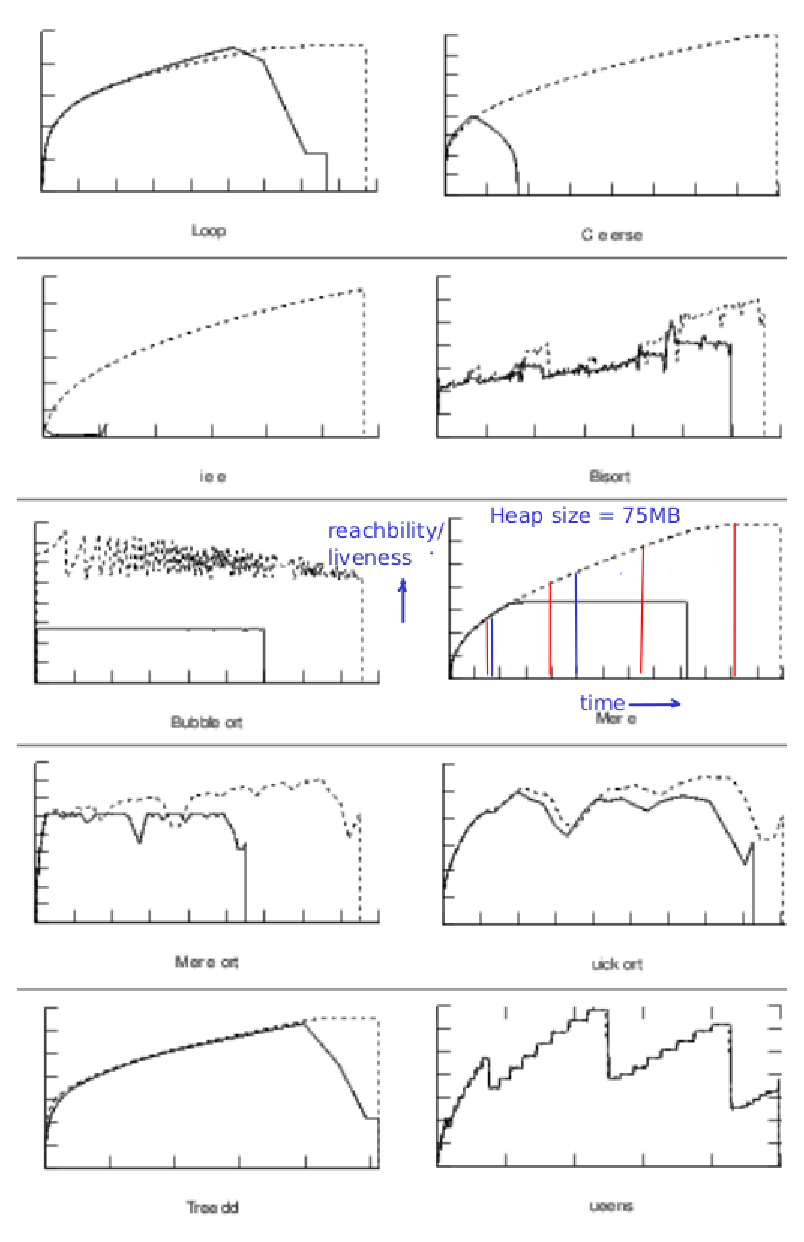
\epsfig{file=memory-usage.eps, width=12cm, height=15cm}}
%% \caption{Memory  usage of  programs. The  solid  lines represents
%%   number of  live cells and the  dashed lines show  the number of
%%   reachable cells.  The red and blue  lines represent invocations
%%   of RGC and  LGC---their heights indicate  the amount of memory
%%   copied.   {\color{red}{Caution:  Figures  are from  a  previous
%%       paper and are being used as placeholder}}}
%% \label{fig:memory-usage} \figrule
%% \end{figure}
%%\clearpage

\section{Related Work} Previous attempts to  increase  the space
efficiency
of functional programs by additional  reclamation of memory fall in two
broad categories. In the first,  the program itself is instrumented to
manage  reclamation and reallocation  without the  aid of  the garbage
collector.    Such    attempts   include:   sharing    analysis   based
reallocation~\cite{jones89compile},                       deforestation
techniques~\cite{wadler88deforest,gill93ashort,chitil99deforest},
methods  based  on   linear  logic~\cite{hofmann00linear}  and  region
analysis~\cite{tofte98region}.   Closer  to  our approach,  there  are
methods   that  enable   the   garbage  collector   to  collect   more
garbage~\cite{inoue88analysis,lee05static}   by
explicitly  nullifying  pointers  that  are not  live.   However,  the
nullification,  done   at  compile  time,   requires  sharing  (alias)
analysis.  Our  method, in contrast, does not  require sharing because
of the availability of the heap  itself at runtime.  To the best of our
knowledge, this is the first  attempt at liveness-based marking of the
heap during garbage collection.  

%% \begin{figure}[t]
%% \centerline{\epsfig{file=lambda.eps, height=4cm, width=7cm}}
%%  \caption{Memory  usage and garbage collection pattern of  {\tt
%% lambda}.}
%% \label{fig:memory-usage-lambda} \figrule
%% \end{figure}

\section{Conclusions}
\label{sec:conclusion}
We  have  defined  a  notion  of liveness  on  structured  data;  this
generalizes classical liveness and strong liveness.  We started with a
general fully context-sensitive analysis  which we proved correct with
respect to  a minefield semantics  (this models the effect  of garbage
collection between every evaluation step).

To  avoid scalability  issues (and  to  avoid performing  part of  the
liveness computation at run time)  we defined an 0-CFA version of this
liveness analysis  in which  demands for function  $f$ at  all calling
contexts are conflated into  a single demand $\sigma_f$.  This enabled
us to treat the liveness equations symbolically obtaining context-free
grammars for liveness at each GC point (calls to user functions and to
$\CONS$).  These were then converted to DFAs for run-time consultation
by  the garbage collector.  Experiments confirm  the precision  of the
analysis.

To obtain performance figures we compared a reachability-based garbage
collector with a liveness-based  collector.  This showed a decrease in
the  number  of  GCs,   more  garbage  collected  per  invocation.   A
significant benefit of LGC is  that programs can run in smaller memory
when compared to  RGC. This is potentially useful  in situations where
memory  is  limited---as with  embedded  systems.  For  a majority  of
programs, the garbage collection times were reduced.

One issue we  highlighted was that while fewer  nodes were marked (and
more garbage collected), sometimes  cons cells could be visited and
traversed  multiple times  with different  sets of  liveness  paths to
explore.  Further work includes  improvements to the classical copying
collector to reduce the cost of this.


%Add graphs for memort usage LGC vs RGC
%Add graphs/table showing the GC times and other statistics

%Mention lower peak memory usage.
%Mention faster GC than full LGC and more garbage collected than RGC.
%Pitch it as sweet spot between full LGC and RGC.
%Future work
%Mention full LGC
%Mention k-liveness, use length example to show 1-liveness is not
sufficient.
%Mention mixed mode GC,
% - doing RGC most of the times and switching to LGC in case RGC fails
to collect any garbage
% - doing LGC most of the times but regularly checking the reachability
of the heap and
% switching to RGC if LGC almost equals RGC

\subsection{References}
\bibliography{fun_hra}{}
\bibliographystyle{abbrv}

Generated by bibtex from your ~.bib file.  Run latex,
then bibtex, then latex twice (to resolve references)
to create the ~.bbl file.  Insert that ~.bbl file into
the .tex source file and comment out
the command \texttt{{\char'134}thebibliography}.
% This next section command marks the start of
% Appendix B, and does not continue the present hierarchy
\section{More Help for the Hardy}
The sig-alternate.cls file itself is chock-full of succinct
and helpful comments.  If you consider yourself a moderately
experienced to expert user of \LaTeX, you may find reading
it useful but please remember not to change it.
%\balancecolumns % GM June 2007
% That's all folks!





% {\color{red}
%   (Note 3.\ includes $e_\mainpgm$ treated as the body of
%   $(\DEFINE\ ({\tt main})\ e_\mainpgm)$.)
% }




%% =======

%------------------------------------------------------------%
%\begin{figure}[t]
  \begin{boxedminipage}{\textwidth}
    \begin{center}
      \raggedright  {\bf  Input:}  Demand $\sigma$ \\
      \raggedright  {\bf  Input:}  Demand Transformer LF \\
      %
      \raggedright{\bf Output:} Modified Liveness Environment Map
      \\
      %  
      \raggedright{\bf Steps:}
      \begin{algorithmic}
        \STATE $M \leftarrow process\_liveness(e, \sigma, LF)$
        \STATE $numargs \leftarrow$ number of arguments in $s$
        \STATE $f \leftarrow$ a new function with $\myvec{x}$ as the argument vector
        
        \FORALL{$l$ in label\_set($e$)} 
        \STATE $var \leftarrow let\_var$ 
        \STATE $rexpr \leftarrow let\_expr$
        \IF {$rexpr$ contains $var$}
        \STATE $L_f \leftarrow process\_liveness (\ f, M[l, x],\ LF)$
        \STATE $le \leftarrow \bigcup_{i=1}^{numargs} x_i.LF_{f}^{i}({\sigma})$
        \ELSE
        \STATE  $le \leftarrow  ref (s,\ \sigma,\ LF)$
        \ENDIF
        \STATE $M[l] = M[l] \bigcup le$
        \ENDFOR
        \RETURN $M$
      \end{algorithmic}
    \end{center}
  \end{boxedminipage}
  \caption{Algorithm for transforming demand for a lazy let}\label{algo:transform-lazy-let} \figrule
\end{figure}

\begin{figure}[t]
  \begin{boxedminipage}{\textwidth}
    \begin{center}
      \raggedright  {\bf  Input:}  Program execution stack  $S$ \\
      \raggedright  {\bf  Input:}  Print stack $P$ \\
      %
      \raggedright{\bf Output:} void \\
      %  
      \raggedright{\bf Steps:}
      \begin{algorithmic}
        \FORALL{$funccall$ in $S$} 
        \STATE $pgm\_pt \leftarrow funccall.return\_pt$
        \FORALL{$var$ in $funccall.varstack$} 
        \STATE $var \leftarrow let\_var$ 
        \STATE $rexpr \leftarrow let\_expr$
        \IF {$rexpr$ contains $var$}
        \STATE $L_f \leftarrow process\_liveness (\ f, M[l, x],\ LF)$
        \STATE $le \leftarrow \bigcup_{i=1}^{numargs} x_i.LF_{f}^{i}({\sigma})$
        \ELSE
        \STATE  $le \leftarrow  ref (s,\ \sigma,\ LF)$
        \ENDIF
        \STATE $M[l] = M[l] \bigcup le$
        \ENDFOR
        \ENDFOR
        \RETURN $M$
      \end{algorithmic}
    \end{center}
  \end{boxedminipage}
  \caption{Algorithm for Liveness based GC}\label{algo:lazy-lgc} \figrule
\end{figure}


\end{document}
